% ==================================================================
%  §11.1  第一型曲线、曲面积分
%  源：徐森林、薛春华《数学分析》第二册，印刷页 297-322
%  底本：PaddleOCR-VL 为主，MinerU 交叉核对
%  约定：全西文标点；\[\] 表行间公式；align*/aligned 表多行；
%        原书「理由写在横线上」用 \reason{}；证明/解以 \qedhere 收 □
%  注意：OCR 常见错误已订正
%        · \int_{a}^{\beta} -> \int_{\alpha}^{\beta}
%        · \int_{c} -> \int_{C}（OCR 把小写 c 当成了积分下标）
%        · \mathrm{c o s} -> \cos；\parallel -> \|；\bullet -> \cdot
%        · 撇号：定义 11.1.1' / 定理 11.1.1' 与前者同号
% ==================================================================
\section{第一型曲线、曲面积分}

在\extref{定义 6.6.1}中给出了可求长曲线的弧长的定义, 进而, \extref{定理 6.6.1}证明了 $C^{1}$ 光滑正则曲线弧长公式为
\[
  s=\int_{\alpha}^{\beta}\sqrt{\left[x^{\prime}(t)\right]^{2}+\left[y^{\prime}(t)\right]^{2}+\left[z^{\prime}(t)\right]^{2}}\,\mathrm{d} t.
\]

在此基础上, 我们来定义可求长曲线 $C$ 的第一型曲线积分.

\begin{definition}\label{def:11.1.1}
设 $U \subset \mathbb{R}^{3}$ 为一区域, 函数 $f: U \to \mathbb{R}$. 可求长曲线 $C \subset U$, 其两个端点分别记为 $A$ 与 $B$. 在 $C$ 上依次取一列点 $\{P^{i} \mid i=0,1,\cdots,m\}$, 使得 $P^{0}=A$, $P^{m}=B$. 称 $\widehat{P^{i-1} P^{i}}$ 为 $C$ 的第 $i$ 段曲线, 令 $\Delta s_{i}=s\left(\widehat{P^{i-1} P^{i}}\right)$ 为 $C$ 的第 $i$ 段曲线的弧长. 在 $\widehat{P^{i-1} P^{i}}$ 上任取一点 $\boldsymbol{\xi}^{i}\ (i=1,2,\cdots,m)$, 如果极限
\[
  \lim _{\max \Delta s_{i} \to 0} \sum_{i=1}^{m} f\left(\boldsymbol{\xi}^{i}\right) \Delta s_{i}
\]
是一个有限数, 并且其值不依赖于点列 $\{P^{i} \mid i=0,1,\cdots,m\}$ 与点 $\boldsymbol{\xi}^{i}$ 在 $\widehat{P^{i-1} P^{i}}$ 上的选择, 那就将这个极限值记为
\[
  \int_{C} f\,\mathrm{d} s, \quad \text{或}\ \int_{C} f(\boldsymbol{x})\,\mathrm{d} s, \quad \text{或}\ \int_{C} f(x, y, z)\,\mathrm{d} s,
\]
称之为函数 $f$ 在 $C$ 上的第一型曲线积分.
\end{definition}

当 $f(x)=1, \forall x \in C$ 时, 显然 $\int_{C} \mathrm{d} s=s(C)$, 即曲线 $C$ 的弧长.

现在来推导计算第一型曲线积分的公式.

\begin{theorem}[$\mathbb{R}^{3}$ 中第一型曲线积分的计算公式]\label{thm:11.1.1}
设 $U \subset \mathbb{R}^{3}$ 为一区域, $C^{1}$ 光滑正则曲线 $C \subset U$ 有参数表示
\[
  \boldsymbol{x}=\boldsymbol{x}(t)=(x(t), y(t), z(t)), \quad t \in[\alpha, \beta],
\]
$f$ 为曲线 $C$ 上的连续函数, 则
\begin{align*}
  \int_{C} f\,\mathrm{d} s &=\int_{\alpha}^{\beta} f \circ \boldsymbol{x}(t)\left\|\boldsymbol{x}^{\prime}(t)\right\| \mathrm{d} t \\
                           &=\int_{\alpha}^{\beta} f(x(t), y(t), z(t)) \sqrt{\left[x^{\prime}(t)\right]^{2}+\left[y^{\prime}(t)\right]^{2}+\left[z^{\prime}(t)\right]^{2}}\,\mathrm{d} t,
\end{align*}
也就是说, 第一型曲线积分可以化成定积分来计算.
\end{theorem}

\begin{proof}
设 $P^{i}=\boldsymbol{x}\left(t_{i}\right)$, $i=0,1,\cdots,m$ 且 $\alpha=t_{0}<t_{1}<\cdots<t_{m-1}<t_{m}=\beta$, $\boldsymbol{\xi}^{i}=\boldsymbol{x}\left(\eta_{i}\right) \in \widehat{P^{i-1} P^{i}}$, $\eta_{i} \in\left[t_{i-1}, t_{i}\right]$, $i=1,2,\cdots,m$. 根据\extref{定理 6.6.1}, 曲线 $C$ 上变点的弧长为
\[
  s(t)=\int_{\alpha}^{t}\left\|\boldsymbol{x}^{\prime}(\tau)\right\| \mathrm{d} \tau.
\]
由此可知,
\begin{align*}
  \Delta s_{i} &=s\left(t_{i}\right)-s\left(t_{i-1}\right)=\int_{t_{i-1}}^{t_{i}}\left\|\boldsymbol{x}^{\prime}(\tau)\right\| \mathrm{d} \tau \\
               &\reason{积分中值定理}\left\|\boldsymbol{x}^{\prime}\left(\zeta_{i}\right)\right\|\left(t_{i}-t_{i-1}\right)=\left\|\boldsymbol{x}^{\prime}\left(\zeta_{i}\right)\right\| \Delta t_{i},
\end{align*}
其中 $\zeta_{i} \in\left[t_{i-1}, t_{i}\right]$, $i=1,2,\cdots,m$. 于是,
\begin{align*}
  \int_{C} f\,\mathrm{d} s &=\lim _{\max \Delta t_{i} \to 0} \sum_{i=1}^{m} f\left(\boldsymbol{\xi}^{i}\right) \Delta s_{i}=\lim _{\max \Delta t_{i} \to 0} \sum_{i=1}^{m} f\left(\boldsymbol{x}\left(\eta_{i}\right)\right)\left\|\boldsymbol{x}^{\prime}\left(\zeta_{i}\right)\right\| \Delta t_{i} \\
                           &\reason{类似\extref{定理 6.1.1}的证明}\lim _{\max \Delta t_{i} \to 0} \sum_{i=1}^{m} f\left(\boldsymbol{x}\left(\eta_{i}\right)\right)\left\|\boldsymbol{x}^{\prime}\left(\eta_{i}\right)\right\| \Delta t_{i} \\
                           &=\int_{\alpha}^{\beta} f \circ \boldsymbol{x}(t)\left\|\boldsymbol{x}^{\prime}(t)\right\| \mathrm{d} t. \qedhere
\end{align*}
\end{proof}

如果空间曲线 $C$ 以直角坐标 $x$ 为参数, $(x, y, z)=(x, y(x), z(x))$, 且 $y(x), z(x)$ 在 $[a, b]$ 上连续可导, 则空间曲线 $C$ 上的第一型曲线积分公式为
\[
  \int_{a}^{b} f(x, y(x), z(x)) \sqrt{1+\left[y^{\prime}(x)\right]^{2}+\left[z^{\prime}(x)\right]^{2}}\,\mathrm{d} x.
\]

类似上面讨论, 或在上述公式中令 $z=z(t)=0$, 则有平面曲线 $C$ 上的第一型曲线积分公式为
\[
  \int_{C} f\,\mathrm{d} s=\int_{\alpha}^{\beta} f(x(t), y(t)) \sqrt{\left[x^{\prime}(t)\right]^{2}+\left[y^{\prime}(t)\right]^{2}}\,\mathrm{d} t.
\]

如果以直角坐标 $x$ 为参数, 即 $(x, y)=(x, y(x))$, 且 $y(x)$ 在 $[a, b]$ 上连续可导, 则平面曲线 $C$ 上的第一型曲线积分公式为
\[
  \int_{C} f\,\mathrm{d} s=\int_{a}^{b} f(x, y(x)) \sqrt{1+\left[y^{\prime}(x)\right]^{2}}\,\mathrm{d} x.
\]

如果平面曲线 $C$ 由极坐标方程
\[
  r=r(\theta), \quad \theta \in[\alpha, \beta]
\]
给出, $r(\theta)$ 连续可导,
\[
  (x, y)=(r(\theta) \cos \theta, r(\theta) \sin \theta),
\]
则
\[
  \left[x^{\prime}(\theta)\right]^{2}+\left[y^{\prime}(\theta)\right]^{2}=r^{2}(\theta)+\left[r^{\prime}(\theta)\right]^{2} \neq 0.
\]
因而平面上曲线 $C$ 的第一型曲线积分公式为
\[
  \int_{C} f\,\mathrm{d} s=\int_{\alpha}^{\beta} f(r \cos \theta, r \sin \theta) \sqrt{r^{2}(\theta)+\left[r^{\prime}(\theta)\right]^{2}}\,\mathrm{d} \theta.
\]

更一般地, 类似\cref{def:11.1.1}, 在 $\mathbb{R}^{n}$ 中引进第一型曲线积分, 并给出第一型曲线积分的计算公式.

\begin{definitionp}\label{def:11.1.1p}
设 $U \subset \mathbb{R}^{n}$ 为一区域, 函数 $f: U \to \mathbb{R}$. 可求长曲线 $C \subset U$, 其两个端点分别记为 $A$ 与 $B$. 在 $C$ 上依次取一列点 $\{P^{i} \mid i=0,1,\cdots,m\}$, 使得 $P^{0}=A$, $P^{m}=B$. 称 $\widehat{P^{i-1} P^{i}}$ 为 $C$ 的第 $i$ 段曲线, 令 $\Delta s_{i}=s\left(\widehat{P^{i-1} P^{i}}\right)$ 为 $C$ 的第 $i$ 段曲线的弧长 ($\mathbb{R}^{n}$ 中曲线弧长的定义与\extref{定义 6.6.1}完全类似). 在 $\widehat{P^{i-1} P^{i}}$ 上任取一点 $\boldsymbol{\xi}^{i}\ (i=1,2,\cdots,m)$, 如果极限
\[
  \lim _{\max \Delta s_{i} \to 0} \sum_{i=1}^{m} f\left(\boldsymbol{\xi}^{i}\right) \Delta s_{i}
\]
是一个有限数, 并且其值不依赖于点列 $\{P^{i} \mid i=0,1,\cdots,m\}$ 与 $\boldsymbol{\xi}^{i}$ 在 $\widehat{P^{i-1} P^{i}}$ 上的选择, 那就将这个极限值记为
\[
  \int_{C} f\,\mathrm{d} s, \quad \text{或}\ \int_{C} f(\boldsymbol{x})\,\mathrm{d} s, \quad \text{或}\ \int_{C} f\left(x_{1}, x_{2}, \cdots, x_{n}\right) \mathrm{d} s,
\]
称之为函数 $f$ 在 $C$ 上的第一型曲线积分.
\end{definitionp}

\begin{theoremp}[$\mathbb{R}^{n}$ 中第一型曲线积分的计算公式]\label{thm:11.1.1p}
设 $U \subset \mathbb{R}^{n}$ 为一区域, $C^{1}$ 光滑曲线 $C \subset U$ 有参数表示
\[
  \boldsymbol{x}=\boldsymbol{x}(t)=\left(x_{1}(t), x_{2}(t), \cdots, x_{n}(t)\right), \quad t \in[\alpha, \beta],
\]
$f$ 为曲线 $C$ 上的连续函数, 则
\begin{align*}
  \int_{C} f\,\mathrm{d} s &=\int_{\alpha}^{\beta} f \circ \boldsymbol{x}(t)\left\|\boldsymbol{x}^{\prime}(t)\right\| \mathrm{d} t \\
                           &=\int_{\alpha}^{\beta} f\left(x_{1}(t), x_{2}(t), \cdots, x_{n}(t)\right) \sqrt{\left[x_{1}^{\prime}(t)\right]^{2}+\left[x_{2}^{\prime}(t)\right]^{2}+\cdots+\left[x_{n}^{\prime}(t)\right]^{2}}\,\mathrm{d} t,
\end{align*}
也就是说, 第一型曲线积分可以化成定积分来计算.
\end{theoremp}

\begin{example}\label{ex:11.1.1}
求圆柱螺线 (\extref{图 6.6.17}) $C:(x, y, z)=(a \cos t, a \sin t, b t)$, $t \in[0,2 \pi]$ 上一段的弧长 $s(C)$.
\end{example}

\begin{solution}
\begin{align*}
  s(C) &=\int_{0}^{2 \pi} \sqrt{\left[x^{\prime}(t)\right]^{2}+\left[y^{\prime}(t)\right]^{2}+\left[z^{\prime}(t)\right]^{2}}\,\mathrm{d} t=\int_{0}^{2 \pi} \sqrt{(-a \sin t)^{2}+(a \cos t)^{2}+b^{2}}\,\mathrm{d} t \\
       &=\sqrt{a^{2}+b^{2}} \int_{0}^{2 \pi} \mathrm{d} t=2 \pi \sqrt{a^{2}+b^{2}}. \qedhere
\end{align*}
\end{solution}

\begin{example}\label{ex:11.1.2}
计算第一型曲线积分 $\int_{C} \frac{z^{2}}{x^{2}+y^{2}}\,\mathrm{d} s$, 其中 $C$ 为圆柱螺线
\[
  (x, y, z)=(a \cos t, a \sin t, b t), \quad t \in[0,2 \pi].
\]
\end{example}

\begin{solution}
\begin{align*}
  \int_{C} \frac{z^{2}}{x^{2}+y^{2}}\,\mathrm{d} s &=\int_{0}^{2 \pi} \frac{z^{2}(t)}{x^{2}(t)+y^{2}(t)} \sqrt{\left[x^{\prime}(t)\right]^{2}+\left[y^{\prime}(t)\right]^{2}+\left[z^{\prime}(t)\right]^{2}}\,\mathrm{d} t \\
  &=\int_{0}^{2 \pi} \frac{(b t)^{2}}{(a \cos t)^{2}+(a \sin t)^{2}} \sqrt{(-a \sin t)^{2}+(a \cos t)^{2}+b^{2}}\,\mathrm{d} t \\
  &=\frac{b^{2}}{a^{2}} \sqrt{a^{2}+b^{2}} \int_{0}^{2 \pi} t^{2}\,\mathrm{d} t=\left(\frac{b}{a}\right)^{2} \sqrt{a^{2}+b^{2}} \cdot \frac{t^{3}}{3}\bigg|_{0} ^{2 \pi} \\
  &=\frac{8}{3}\left(\frac{b}{a}\right)^{2} \sqrt{a^{2}+b^{2}}\, \pi^{3}. \qedhere
\end{align*}
\end{solution}

\begin{example}\label{ex:11.1.3}
计算第一型曲线积分 $\int_{C} x y\,\mathrm{d} s$, 其中 $C$ 为球面 $x^{2}+y^{2}+z^{2}=a^{2}$ 与平面 $x+y+z=0$ 交成的圆周.
\end{example}

\begin{solution}[解法 1 (常规算法)]
由于 $C$ 所在平面 $x+y+z=0$ 的法向量为 $(1,1,1)$. 我们取
\[
  \left\{\begin{aligned}
    \boldsymbol{e}_{1} &=\frac{1}{\sqrt{6}}(1,-2,1), \\
    \boldsymbol{e}_{2} &=\frac{1}{\sqrt{2}}(1,0,-1), \\
    \boldsymbol{e}_{3} &=\frac{1}{\sqrt{3}}(1,1,1),
  \end{aligned}\right.
\]
这是三个互相正交的单位向量, $\boldsymbol{e}_{1}$ 与 $\boldsymbol{e}_{2}$ 张成 $C$ 所在的平面 $x+y+z=0$. 因此, $C$ 的参数表示为 (\cref{fig:11.1.1})
\begin{align*}
  (x, y, z)=\boldsymbol{x}=\boldsymbol{x}(\theta) &=a\left(\cos \theta\, \boldsymbol{e}_{1}+\sin \theta\, \boldsymbol{e}_{2}\right) \\
  &=a\left[\frac{1}{\sqrt{6}} \cos \theta(1,-2,1)+\frac{1}{\sqrt{2}} \sin \theta(1,0,-1)\right] \\
  &=a\left(\frac{1}{\sqrt{6}} \cos \theta+\frac{1}{\sqrt{2}} \sin \theta,\ -\frac{2}{\sqrt{6}} \cos \theta,\ \frac{1}{\sqrt{6}} \cos \theta-\frac{1}{\sqrt{2}} \sin \theta\right).
\end{align*}

\begin{figure}[htbp]
  \centering
  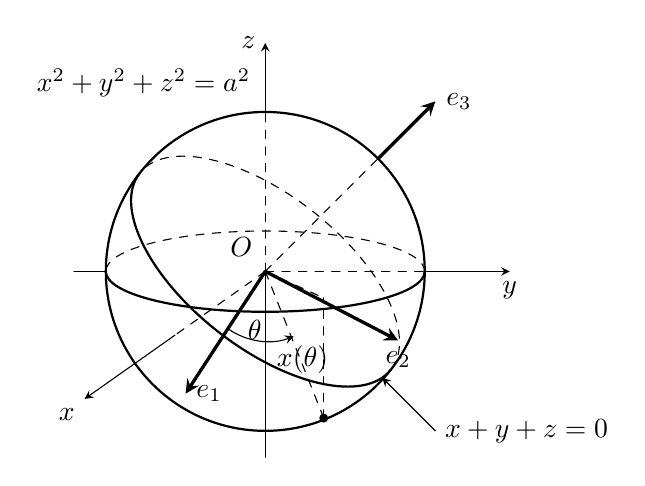
\begin{tikzpicture}[scale=1.35, >=stealth, line cap=round, line join=round]
    % 球面外轮廓圆
    \draw[thick] (0,0) circle (1.5);
    
    % 赤道椭圆: 前半实线，后半虚线
    \draw[dashed] (1.5,0) arc (0:180:1.5 and 0.38);
    \draw[thick] (-1.5,0) arc (180:360:1.5 and 0.38);
    
    % 坐标轴: 原点 O 在球心
    % z 轴向上
    \draw[dashed] (0,0) -- (0,1.5);
    \draw[->] (0,1.5) -- (0,2.15) node[left] {$z$};
    \draw (0,0) -- (0,-1.75);
    
    % y 轴向右水平
    \draw[dashed] (0,0) -- (1.5,0);
    \draw[->] (1.5,0) -- (2.3,0) node[below] {$y$};
    \draw (-1.8,0) -- (-1.5,0);
    
    % x 轴向左前斜下方 (约 215 度)
    \draw[dashed] (0,0) -- (-0.85,-0.6);
    \draw[->] (-0.85,-0.6) -- (-1.7,-1.2) node[below left] {$x$};
    
    % 原点标签 O
    \node[above left] at (-0.03,0.05) {$O$};
    
    % 平面 x+y+z=0 截球的大圆椭圆 C:
    % 原书显示为一个倾斜的大椭圆，长轴约沿 -40°/140° 方向，前半实线，后半虚线
    \begin{scope}[rotate=-38]
      \draw[thick] (-1.5,0) arc (180:360:1.5 and 0.72);
      \draw[dashed] (1.5,0) arc (0:180:1.5 and 0.72);
    \end{scope}
    
    % 基底向量 e_3 (法向量 n0 方向，即 (1,1,1) 方向，在图中指向右上方)
    \draw[dashed] (0,0) -- (1.06,1.06);
    \draw[->,very thick] (1.06,1.06) -- (1.6,1.6) node[right] {$\boldsymbol{e}_{3}$};
    
    % 截面平面内正交基底 e_1 与 e_2:
    % e_1 指向左下方
    \draw[->,very thick] (0,0) -- (-0.75,-1.15) node[right] {$\boldsymbol{e}_{1}$};
    
    % e_2 指向右下方
    \draw[->,very thick] (0,0) -- (1.25,-0.65) node[below] {$\boldsymbol{e}_{2}$};
    
    % 在 C 上取点 x(theta):
    \draw[dashed] (0,0) -- (0.55,-1.38);
    \fill (0.55,-1.38) circle (1.2pt);
    \node[above] at (0.35,-1.05) {$\boldsymbol{x}(\theta)$};
    
    % theta 角弧线 (从 e_1 到 x(theta))
    \draw[->] (-0.35,-0.54) arc (-125:-68:0.65);
    \node at (-0.1,-0.55) {$\theta$};
    
    % 竖直投影辅助虚线: 从 x(theta) 向上做垂直辅助线到赤道面
    \draw[dashed] (0.55,-1.38) -- (0.55,-0.25);
    \draw[dashed] (0,0) -- (0.55,-0.25);
    
    % 公式标注:
    % 左上角: x^2 + y^2 + z^2 = a^2
    \node[above left] at (-0.05,1.55) {$x^{2}+y^{2}+z^{2}=a^{2}$};
    % 右下角: x + y + z = 0 指向截面大圆
    \draw[<-] (1.1,-1.0) -- (1.6,-1.5) node[right] {$x+y+z=0$};
  \end{tikzpicture}
  \caption{}\label{fig:11.1.1}
\end{figure}

于是, 半径为 $a$ 的圆 $C$ 的弧长元为 $\mathrm{d} s=a\,\mathrm{d} \theta$, 或者
\[
  \mathrm{d} s=\left\|\boldsymbol{x}^{\prime}(\theta)\right\| \mathrm{d} \theta=\left\|a\left(-\sin \theta\, \boldsymbol{e}_{1}+\cos \theta\, \boldsymbol{e}_{2}\right)\right\|=a\,\mathrm{d} \theta.
\]
因此, 第一型曲线积分
\begin{align*}
  \int_{C} x y\,\mathrm{d} s &=\int_{0}^{2 \pi} a\left(\frac{1}{\sqrt{6}} \cos \theta+\frac{1}{\sqrt{2}} \sin \theta\right) \cdot a\left(-\frac{2}{\sqrt{6}} \cos \theta\right) \cdot a\,\mathrm{d} \theta \\
  &=a^{3} \int_{0}^{2 \pi}\left(-\frac{2}{6} \cos ^{2} \theta-\sqrt{\frac{2}{6}} \sin \theta \cos \theta\right) \mathrm{d} \theta \\
  &=-\frac{1}{3} a^{3} \int_{0}^{2 \pi} \cos ^{2} \theta\,\mathrm{d} \theta=-\frac{1}{3} a^{3} \int_{0}^{2 \pi} \frac{1+\cos 2 \theta}{2}\,\mathrm{d} \theta \\
  &=-\frac{1}{3} a^{3}\left(\pi+\frac{1}{2} \sin 2 \theta\bigg|_{0} ^{2 \pi}\right)=-\frac{1}{3} \pi a^{3}. \qedhere
\end{align*}
\end{solution}

\begin{solution}[解法 2 (利用对称性)]
由代数与几何两方面的对称性, 有
\[
  \int_{C} x y\,\mathrm{d} s=\int_{C} y z\,\mathrm{d} s=\int_{C} z x\,\mathrm{d} s,
\]
所以,
\begin{align*}
  \int_{C} x y\,\mathrm{d} s &=\frac{1}{3} \int_{C}(x y+y z+z x)\,\mathrm{d} s \\
  &=\frac{1}{6} \int_{C}\left[(x+y+z)^{2}-\left(x^{2}+y^{2}+z^{2}\right)\right] \mathrm{d} s \\
  &=\frac{1}{6} \int_{C}\left(0^{2}-a^{2}\right) \mathrm{d} s=-\frac{1}{6} a^{2} s(C)=-\frac{1}{6} a^{2} \cdot 2 \pi a=-\frac{1}{3} \pi a^{3}. \qedhere
\end{align*}
\end{solution}

上面讨论的第一型曲线积分与曲线的弧长关系密切. 第一型曲面积分与曲面面积的关联也很密切. 因此, 我们必须从曲面的面积讲起.

许多平面图形的面积计算公式, 早在 Euclid 的\textit{几何原本}出现之前就已经建立起来了. 特别是平面多边形的面积计算, 也许是更早一些的事. 对于一般的平面上有界点集的面积, 在\extref{定义 10.2.2}中已经通过二重积分给出.

多面体的表面是由一些平面多边形组成的, 其表面积就是这些平面多边形的面积之和, 因此多面体的表面积的计算就被认为是解决了. 对于弯曲的曲面, 它的面积, 人们想到用内接于该曲面的若干平面三角形组成的图形 (称为折面) 的表面积来逼近是很自然的事. 曲线的弧长正是用内接于该曲线的连续折线的长度来逼近的. 对于弯曲的曲面抱有类似的希望又有什么不合理的呢? 但是, 19 世纪末, H. A. Schwarz 给出了一个著名的例子说明, 即使对于非常简单的曲面, 这种想法也是行不通的.

考虑一个底半径为 $1$, 高为 $1$ 的直圆柱面 $\Sigma$. 若将 $\Sigma$ 沿一条母线剪开, 然后将它平铺在平面上, 就变成了一个边长为 $1$ 与 $2 \pi$ 的矩形. 这个矩形的面积等于 $2 \pi$, 因此 $\Sigma$ 的表面积就应当等于 $2 \pi$. Schwarz 考虑用折面来逼近这个直圆柱面: 用与母线垂直的, 间隔均匀的 $m+1$ 张平面去分割这个直圆柱面, 截出 $m+1$ 个圆周. 然后在每个这样的圆周上, 用 $n$ 个分点将它等分. 这些分点是这样分布的: 上一个圆周上的分点对最靠近它的下一圆周的垂直投影与下一圆周上的相邻两个分点有相等的距离. \cref{fig:11.1.2}中的分点 $A$ 与 $B$, $C$ 就代表这种关系.

\begin{figure}[htbp]
  \centering
  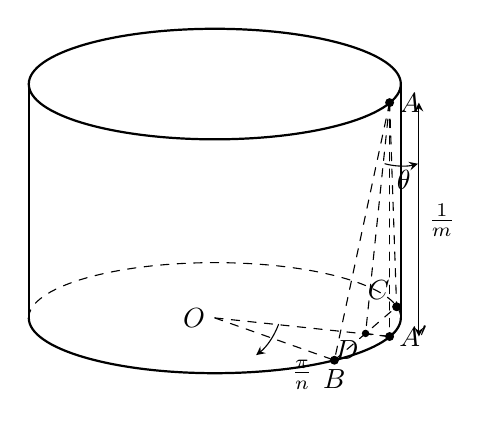
\begin{tikzpicture}[scale=1.35, >=stealth, line cap=round, line join=round]
    % 圆柱顶底面椭圆
    \draw[thick] (0,2.2) ellipse (1.75 and 0.52);
    \draw[dashed] (-1.75,0) arc (180:0:1.75 and 0.52);
    \draw[thick] (-1.75,0) arc (180:360:1.75 and 0.52);
    % 两侧竖直母线
    \draw[thick] (-1.75,2.2) -- (-1.75,0);
    \draw[thick] (1.75,2.2) -- (1.75,0);
    
    % 底面圆心 O
    \coordinate (Obot) at (0,0);
    \node[left] at (Obot) {$O$};
    
    % 顶面点 A
    \coordinate (A) at (1.644, 2.025);
    \fill (A) circle (1.2pt) node[right] {$A$};
    
    % 底面对应投影点 A'
    \coordinate (Ap) at (1.644, -0.175);
    \fill (Ap) circle (1.2pt) node[right] {$A'$};
    \draw[dashed] (A) -- (Ap);
    
    % 高度 1/m
    \draw[<->] (1.92, 2.025) -- (1.92, -0.175);
    \node[right] at (1.92, 0.92) {$\frac{1}{m}$};
    
    % 底面相邻分点 B 和 C
    \coordinate (B) at (1.125, -0.398);
    \coordinate (C) at (1.710, 0.105);
    \fill (B) circle (1.2pt) node[below] {$B$};
    \fill (C) circle (1.2pt) node[above left=-1pt] {$C$};
    
    % 弦 BC 的中点 D
    \coordinate (D) at (1.418, -0.146);
    \fill (D) circle (1.0pt) node[below left=-1pt] {$D$};
    \draw[dashed] (B) -- (C);
    
    % 从 O 连虚线到 A' 和 B
    \draw[dashed] (Obot) -- (Ap);
    \draw[dashed] (Obot) -- (B);
    
    % 夹角 pi/n 在 O 处引出
    \draw[->] (0.60, -0.06) arc (-20:-52:0.65);
    \node[below=1pt] at (0.82, -0.28) {$\frac{\pi}{n}$};
    
    % 连线 A'D
    \draw[dashed] (Ap) -- (D);
    
    % 三角形 ABC 及其在侧面的斜向连线
    \draw[dashed] (A) -- (B);
    \draw[dashed] (A) -- (C);
    \draw[dashed] (A) -- (D);
    
    % 夹角 theta (AA' 与 AD 在 A 点的夹角)
    \draw[->] (1.60, 1.45) arc (-105:-75:0.6);
    \node[right] at (1.62, 1.30) {$\theta$};
  \end{tikzpicture}
  \caption{}\label{fig:11.1.2}
\end{figure}

再将 $A, B, C$ 三点连成一个三角形, 并且设想所有的有这种关系的三个分点都被这样地连成了三角形, 造成了\cref{fig:11.1.3}那样的模型, 它是一个内接于直圆柱面的折面. 这个折面由 $2 m n$ 个全等的三角形组成.

在\cref{fig:11.1.2}中, $\angle B O A^{\prime}=\frac{\pi}{n}$, 从而 $A^{\prime} D=1-\cos \frac{\pi}{n}$, 所以,
\begin{align*}
  A D &=\sqrt{A^{\prime} A^{2}+A^{\prime} D^{2}} \\
      &=\sqrt{\left(\frac{1}{m}\right)^{2}+\left(1-\cos \frac{\pi}{n}\right)^{2}}.
\end{align*}

于是, 三角形 $A B C$ 的面积为
\begin{align*}
  \frac{1}{2} B C \cdot A D &=B D \cdot A D \\
                            &=\sin \frac{\pi}{n} \sqrt{\left(\frac{1}{m}\right)^{2}+\left(1-\cos \frac{\pi}{n}\right)^{2}}.
\end{align*}

\begin{figure}[htbp]
  \centering
  \begin{tikzpicture}[scale=1.1, >=stealth, line cap=round, line join=round]
    \draw[dashed, thin, black!65] (1.516,-1.833) -- (1.690,-1.275);
    \draw[dashed, thin, black!65] (1.750,-1.754) -- (1.690,-1.275);
    \draw[dashed, thin, black!65] (1.750,-1.754) -- (1.237,-1.204);
    \draw[dashed, thin, black!65] (1.516,-1.675) -- (1.237,-1.204);
    \draw[dashed, thin, black!65] (1.516,-1.675) -- (0.453,-1.163);
    \draw[dashed, thin, black!65] (0.875,-1.617) -- (0.453,-1.163);
    \draw[dashed, thin, black!65] (0.875,-1.617) -- (-0.453,-1.163);
    \draw[dashed, thin, black!65] (0.000,-1.596) -- (-0.453,-1.163);
    \draw[dashed, thin, black!65] (0.000,-1.596) -- (-1.237,-1.204);
    \draw[dashed, thin, black!65] (-0.875,-1.617) -- (-1.237,-1.204);
    \draw[dashed, thin, black!65] (-0.875,-1.617) -- (-1.690,-1.275);
    \draw[dashed, thin, black!65] (-1.516,-1.675) -- (-1.690,-1.275);
    \draw[dashed, thin, black!65] (-1.516,-1.675) -- (-1.690,-1.356);
    \draw[dashed, thin, black!65] (1.690,-1.275) -- (1.750,-0.877);
    \draw[dashed, thin, black!65] (1.690,-1.275) -- (1.516,-0.798);
    \draw[dashed, thin, black!65] (1.237,-1.204) -- (1.516,-0.798);
    \draw[dashed, thin, black!65] (1.237,-1.204) -- (0.875,-0.741);
    \draw[dashed, thin, black!65] (0.453,-1.163) -- (0.875,-0.741);
    \draw[dashed, thin, black!65] (0.453,-1.163) -- (0.000,-0.719);
    \draw[dashed, thin, black!65] (-0.453,-1.163) -- (0.000,-0.719);
    \draw[dashed, thin, black!65] (-0.453,-1.163) -- (-0.875,-0.741);
    \draw[dashed, thin, black!65] (-1.237,-1.204) -- (-0.875,-0.741);
    \draw[dashed, thin, black!65] (-1.237,-1.204) -- (-1.516,-0.798);
    \draw[dashed, thin, black!65] (-1.690,-1.275) -- (-1.516,-0.798);
    \draw[dashed, thin, black!65] (-1.690,-1.275) -- (-1.750,-0.877);
    \draw[dashed, thin, black!65] (1.516,-0.956) -- (1.690,-0.398);
    \draw[dashed, thin, black!65] (1.750,-0.877) -- (1.690,-0.398);
    \draw[dashed, thin, black!65] (1.750,-0.877) -- (1.237,-0.327);
    \draw[dashed, thin, black!65] (1.516,-0.798) -- (1.237,-0.327);
    \draw[dashed, thin, black!65] (1.516,-0.798) -- (0.453,-0.286);
    \draw[dashed, thin, black!65] (0.875,-0.741) -- (0.453,-0.286);
    \draw[dashed, thin, black!65] (0.875,-0.741) -- (-0.453,-0.286);
    \draw[dashed, thin, black!65] (0.000,-0.719) -- (-0.453,-0.286);
    \draw[dashed, thin, black!65] (0.000,-0.719) -- (-1.237,-0.327);
    \draw[dashed, thin, black!65] (-0.875,-0.741) -- (-1.237,-0.327);
    \draw[dashed, thin, black!65] (-0.875,-0.741) -- (-1.690,-0.398);
    \draw[dashed, thin, black!65] (-1.516,-0.798) -- (-1.690,-0.398);
    \draw[dashed, thin, black!65] (-1.516,-0.798) -- (-1.690,-0.479);
    \draw[dashed, thin, black!65] (1.690,-0.398) -- (1.750,0.000);
    \draw[dashed, thin, black!65] (1.690,-0.398) -- (1.516,0.079);
    \draw[dashed, thin, black!65] (1.237,-0.327) -- (1.516,0.079);
    \draw[dashed, thin, black!65] (1.237,-0.327) -- (0.875,0.136);
    \draw[dashed, thin, black!65] (0.453,-0.286) -- (0.875,0.136);
    \draw[dashed, thin, black!65] (0.453,-0.286) -- (0.000,0.157);
    \draw[dashed, thin, black!65] (-0.453,-0.286) -- (0.000,0.157);
    \draw[dashed, thin, black!65] (-0.453,-0.286) -- (-0.875,0.136);
    \draw[dashed, thin, black!65] (-1.237,-0.327) -- (-0.875,0.136);
    \draw[dashed, thin, black!65] (-1.237,-0.327) -- (-1.516,0.079);
    \draw[dashed, thin, black!65] (-1.690,-0.398) -- (-1.516,0.079);
    \draw[dashed, thin, black!65] (-1.690,-0.398) -- (-1.750,0.000);
    \draw[dashed, thin, black!65] (1.516,-0.079) -- (1.690,0.479);
    \draw[dashed, thin, black!65] (1.750,0.000) -- (1.690,0.479);
    \draw[dashed, thin, black!65] (1.750,0.000) -- (1.237,0.550);
    \draw[dashed, thin, black!65] (1.516,0.079) -- (1.237,0.550);
    \draw[dashed, thin, black!65] (1.516,0.079) -- (0.453,0.591);
    \draw[dashed, thin, black!65] (0.875,0.136) -- (0.453,0.591);
    \draw[dashed, thin, black!65] (0.875,0.136) -- (-0.453,0.591);
    \draw[dashed, thin, black!65] (0.000,0.157) -- (-0.453,0.591);
    \draw[dashed, thin, black!65] (0.000,0.157) -- (-1.237,0.550);
    \draw[dashed, thin, black!65] (-0.875,0.136) -- (-1.237,0.550);
    \draw[dashed, thin, black!65] (-0.875,0.136) -- (-1.690,0.479);
    \draw[dashed, thin, black!65] (-1.516,0.079) -- (-1.690,0.479);
    \draw[dashed, thin, black!65] (-1.516,0.079) -- (-1.690,0.398);
    \draw[dashed, thin, black!65] (1.690,0.479) -- (1.750,0.877);
    \draw[dashed, thin, black!65] (1.690,0.479) -- (1.516,0.956);
    \draw[dashed, thin, black!65] (1.237,0.550) -- (1.516,0.956);
    \draw[dashed, thin, black!65] (1.237,0.550) -- (0.875,1.013);
    \draw[dashed, thin, black!65] (0.453,0.591) -- (0.875,1.013);
    \draw[dashed, thin, black!65] (0.453,0.591) -- (0.000,1.034);
    \draw[dashed, thin, black!65] (-0.453,0.591) -- (0.000,1.034);
    \draw[dashed, thin, black!65] (-0.453,0.591) -- (-0.875,1.013);
    \draw[dashed, thin, black!65] (-1.237,0.550) -- (-0.875,1.013);
    \draw[dashed, thin, black!65] (-1.237,0.550) -- (-1.516,0.956);
    \draw[dashed, thin, black!65] (-1.690,0.479) -- (-1.516,0.956);
    \draw[dashed, thin, black!65] (-1.690,0.479) -- (-1.750,0.877);
    \draw[dashed, thin, black!65] (1.516,0.798) -- (1.690,1.356);
    \draw[dashed, thin, black!65] (1.750,0.877) -- (1.690,1.356);
    \draw[dashed, thin, black!65] (1.750,0.877) -- (1.237,1.427);
    \draw[dashed, thin, black!65] (1.516,0.956) -- (1.237,1.427);
    \draw[dashed, thin, black!65] (1.516,0.956) -- (0.453,1.467);
    \draw[dashed, thin, black!65] (0.875,1.013) -- (0.453,1.467);
    \draw[dashed, thin, black!65] (0.875,1.013) -- (-0.453,1.467);
    \draw[dashed, thin, black!65] (0.000,1.034) -- (-0.453,1.467);
    \draw[dashed, thin, black!65] (0.000,1.034) -- (-1.237,1.427);
    \draw[dashed, thin, black!65] (-0.875,1.013) -- (-1.237,1.427);
    \draw[dashed, thin, black!65] (-0.875,1.013) -- (-1.690,1.356);
    \draw[dashed, thin, black!65] (-1.516,0.956) -- (-1.690,1.356);
    \draw[dashed, thin, black!65] (-1.516,0.956) -- (-1.690,1.275);
    \draw[dashed, thin, black!65] (1.690,1.356) -- (1.750,1.754);
    \draw[dashed, thin, black!65] (1.690,1.356) -- (1.516,1.833);
    \draw[dashed, thin, black!65] (1.237,1.427) -- (1.516,1.833);
    \draw[dashed, thin, black!65] (1.237,1.427) -- (0.875,1.890);
    \draw[dashed, thin, black!65] (0.453,1.467) -- (0.875,1.890);
    \draw[dashed, thin, black!65] (0.453,1.467) -- (0.000,1.911);
    \draw[dashed, thin, black!65] (-0.453,1.467) -- (0.000,1.911);
    \draw[dashed, thin, black!65] (-0.453,1.467) -- (-0.875,1.890);
    \draw[dashed, thin, black!65] (-1.237,1.427) -- (-0.875,1.890);
    \draw[dashed, thin, black!65] (-1.237,1.427) -- (-1.516,1.833);
    \draw[dashed, thin, black!65] (-1.690,1.356) -- (-1.516,1.833);
    \draw[dashed, thin, black!65] (-1.690,1.356) -- (-1.750,1.754);
    \draw[dashed, thin, black!65] (1.750,-1.754) -- (1.516,-1.675);
    \draw[dashed, thin, black!65] (1.516,-1.675) -- (0.875,-1.617);
    \draw[dashed, thin, black!65] (0.875,-1.617) -- (0.000,-1.596);
    \draw[dashed, thin, black!65] (0.000,-1.596) -- (-0.875,-1.617);
    \draw[dashed, thin, black!65] (-0.875,-1.617) -- (-1.516,-1.675);
    \draw[dashed, thin, black!65] (-1.516,-1.675) -- (-1.750,-1.754);
    \draw[dashed, thin, black!65] (1.690,-1.356) -- (1.690,-1.275);
    \draw[dashed, thin, black!65] (1.690,-1.275) -- (1.237,-1.204);
    \draw[dashed, thin, black!65] (1.237,-1.204) -- (0.453,-1.163);
    \draw[dashed, thin, black!65] (0.453,-1.163) -- (-0.453,-1.163);
    \draw[dashed, thin, black!65] (-0.453,-1.163) -- (-1.237,-1.204);
    \draw[dashed, thin, black!65] (-1.237,-1.204) -- (-1.690,-1.275);
    \draw[dashed, thin, black!65] (-1.690,-1.275) -- (-1.690,-1.356);
    \draw[dashed, thin, black!65] (1.750,-0.877) -- (1.516,-0.798);
    \draw[dashed, thin, black!65] (1.516,-0.798) -- (0.875,-0.741);
    \draw[dashed, thin, black!65] (0.875,-0.741) -- (0.000,-0.719);
    \draw[dashed, thin, black!65] (0.000,-0.719) -- (-0.875,-0.741);
    \draw[dashed, thin, black!65] (-0.875,-0.741) -- (-1.516,-0.798);
    \draw[dashed, thin, black!65] (-1.516,-0.798) -- (-1.750,-0.877);
    \draw[dashed, thin, black!65] (1.690,-0.479) -- (1.690,-0.398);
    \draw[dashed, thin, black!65] (1.690,-0.398) -- (1.237,-0.327);
    \draw[dashed, thin, black!65] (1.237,-0.327) -- (0.453,-0.286);
    \draw[dashed, thin, black!65] (0.453,-0.286) -- (-0.453,-0.286);
    \draw[dashed, thin, black!65] (-0.453,-0.286) -- (-1.237,-0.327);
    \draw[dashed, thin, black!65] (-1.237,-0.327) -- (-1.690,-0.398);
    \draw[dashed, thin, black!65] (-1.690,-0.398) -- (-1.690,-0.479);
    \draw[dashed, thin, black!65] (1.750,0.000) -- (1.516,0.079);
    \draw[dashed, thin, black!65] (1.516,0.079) -- (0.875,0.136);
    \draw[dashed, thin, black!65] (0.875,0.136) -- (0.000,0.157);
    \draw[dashed, thin, black!65] (0.000,0.157) -- (-0.875,0.136);
    \draw[dashed, thin, black!65] (-0.875,0.136) -- (-1.516,0.079);
    \draw[dashed, thin, black!65] (-1.516,0.079) -- (-1.750,0.000);
    \draw[dashed, thin, black!65] (1.690,0.398) -- (1.690,0.479);
    \draw[dashed, thin, black!65] (1.690,0.479) -- (1.237,0.550);
    \draw[dashed, thin, black!65] (1.237,0.550) -- (0.453,0.591);
    \draw[dashed, thin, black!65] (0.453,0.591) -- (-0.453,0.591);
    \draw[dashed, thin, black!65] (-0.453,0.591) -- (-1.237,0.550);
    \draw[dashed, thin, black!65] (-1.237,0.550) -- (-1.690,0.479);
    \draw[dashed, thin, black!65] (-1.690,0.479) -- (-1.690,0.398);
    \draw[dashed, thin, black!65] (1.750,0.877) -- (1.516,0.956);
    \draw[dashed, thin, black!65] (1.516,0.956) -- (0.875,1.013);
    \draw[dashed, thin, black!65] (0.875,1.013) -- (0.000,1.034);
    \draw[dashed, thin, black!65] (0.000,1.034) -- (-0.875,1.013);
    \draw[dashed, thin, black!65] (-0.875,1.013) -- (-1.516,0.956);
    \draw[dashed, thin, black!65] (-1.516,0.956) -- (-1.750,0.877);
    \draw[dashed, thin, black!65] (1.690,1.275) -- (1.690,1.356);
    \draw[dashed, thin, black!65] (1.690,1.356) -- (1.237,1.427);
    \draw[dashed, thin, black!65] (1.237,1.427) -- (0.453,1.467);
    \draw[dashed, thin, black!65] (0.453,1.467) -- (-0.453,1.467);
    \draw[dashed, thin, black!65] (-0.453,1.467) -- (-1.237,1.427);
    \draw[dashed, thin, black!65] (-1.237,1.427) -- (-1.690,1.356);
    \draw[dashed, thin, black!65] (-1.690,1.356) -- (-1.690,1.275);
    \draw[dashed, thin, black!65] (1.750,1.754) -- (1.516,1.833);
    \draw[dashed, thin, black!65] (1.516,1.833) -- (0.875,1.890);
    \draw[dashed, thin, black!65] (0.875,1.890) -- (0.000,1.911);
    \draw[dashed, thin, black!65] (0.000,1.911) -- (-0.875,1.890);
    \draw[dashed, thin, black!65] (-0.875,1.890) -- (-1.516,1.833);
    \draw[dashed, thin, black!65] (-1.516,1.833) -- (-1.750,1.754);
    \draw[thick] (0.000,-1.911) -- (0.453,-1.467);
    \draw[thick] (0.000,-1.911) -- (1.237,-1.427);
    \draw[thick] (0.875,-1.890) -- (1.237,-1.427);
    \draw[thick] (0.875,-1.890) -- (1.690,-1.356);
    \draw[thick] (1.516,-1.833) -- (1.690,-1.356);
    \draw[thick] (1.516,-1.833) -- (1.690,-1.275);
    \draw[thick] (1.750,-1.754) -- (1.690,-1.275);
    \draw[thick] (1.750,-1.754) -- (1.237,-1.204);
    \draw[thick] (-1.516,-1.675) -- (-1.690,-1.356);
    \draw[thick] (-1.750,-1.754) -- (-1.690,-1.356);
    \draw[thick] (-1.750,-1.754) -- (-1.237,-1.427);
    \draw[thick] (-1.516,-1.833) -- (-1.237,-1.427);
    \draw[thick] (-1.516,-1.833) -- (-0.453,-1.467);
    \draw[thick] (-0.875,-1.890) -- (-0.453,-1.467);
    \draw[thick] (-0.875,-1.890) -- (0.453,-1.467);
    \draw[thick] (0.453,-1.467) -- (0.000,-1.034);
    \draw[thick] (0.453,-1.467) -- (0.875,-1.013);
    \draw[thick] (1.237,-1.427) -- (0.875,-1.013);
    \draw[thick] (1.237,-1.427) -- (1.516,-0.956);
    \draw[thick] (1.690,-1.356) -- (1.516,-0.956);
    \draw[thick] (1.690,-1.356) -- (1.750,-0.877);
    \draw[thick] (1.690,-1.275) -- (1.750,-0.877);
    \draw[thick] (-1.690,-1.275) -- (-1.750,-0.877);
    \draw[thick] (-1.690,-1.356) -- (-1.750,-0.877);
    \draw[thick] (-1.690,-1.356) -- (-1.516,-0.956);
    \draw[thick] (-1.237,-1.427) -- (-1.516,-0.956);
    \draw[thick] (-1.237,-1.427) -- (-0.875,-1.013);
    \draw[thick] (-0.453,-1.467) -- (-0.875,-1.013);
    \draw[thick] (-0.453,-1.467) -- (0.000,-1.034);
    \draw[thick] (0.000,-1.034) -- (0.453,-0.591);
    \draw[thick] (0.000,-1.034) -- (1.237,-0.550);
    \draw[thick] (0.875,-1.013) -- (1.237,-0.550);
    \draw[thick] (0.875,-1.013) -- (1.690,-0.479);
    \draw[thick] (1.516,-0.956) -- (1.690,-0.479);
    \draw[thick] (1.516,-0.956) -- (1.690,-0.398);
    \draw[thick] (1.750,-0.877) -- (1.690,-0.398);
    \draw[thick] (1.750,-0.877) -- (1.237,-0.327);
    \draw[thick] (-1.516,-0.798) -- (-1.690,-0.479);
    \draw[thick] (-1.750,-0.877) -- (-1.690,-0.479);
    \draw[thick] (-1.750,-0.877) -- (-1.237,-0.550);
    \draw[thick] (-1.516,-0.956) -- (-1.237,-0.550);
    \draw[thick] (-1.516,-0.956) -- (-0.453,-0.591);
    \draw[thick] (-0.875,-1.013) -- (-0.453,-0.591);
    \draw[thick] (-0.875,-1.013) -- (0.453,-0.591);
    \draw[thick] (0.453,-0.591) -- (0.000,-0.157);
    \draw[thick] (0.453,-0.591) -- (0.875,-0.136);
    \draw[thick] (1.237,-0.550) -- (0.875,-0.136);
    \draw[thick] (1.237,-0.550) -- (1.516,-0.079);
    \draw[thick] (1.690,-0.479) -- (1.516,-0.079);
    \draw[thick] (1.690,-0.479) -- (1.750,0.000);
    \draw[thick] (1.690,-0.398) -- (1.750,0.000);
    \draw[thick] (-1.690,-0.398) -- (-1.750,0.000);
    \draw[thick] (-1.690,-0.479) -- (-1.750,0.000);
    \draw[thick] (-1.690,-0.479) -- (-1.516,-0.079);
    \draw[thick] (-1.237,-0.550) -- (-1.516,-0.079);
    \draw[thick] (-1.237,-0.550) -- (-0.875,-0.136);
    \draw[thick] (-0.453,-0.591) -- (-0.875,-0.136);
    \draw[thick] (-0.453,-0.591) -- (0.000,-0.157);
    \draw[thick] (0.000,-0.157) -- (0.453,0.286);
    \draw[thick] (0.000,-0.157) -- (1.237,0.327);
    \draw[thick] (0.875,-0.136) -- (1.237,0.327);
    \draw[thick] (0.875,-0.136) -- (1.690,0.398);
    \draw[thick] (1.516,-0.079) -- (1.690,0.398);
    \draw[thick] (1.516,-0.079) -- (1.690,0.479);
    \draw[thick] (1.750,0.000) -- (1.690,0.479);
    \draw[thick] (1.750,0.000) -- (1.237,0.550);
    \draw[thick] (-1.516,0.079) -- (-1.690,0.398);
    \draw[thick] (-1.750,0.000) -- (-1.690,0.398);
    \draw[thick] (-1.750,0.000) -- (-1.237,0.327);
    \draw[thick] (-1.516,-0.079) -- (-1.237,0.327);
    \draw[thick] (-1.516,-0.079) -- (-0.453,0.286);
    \draw[thick] (-0.875,-0.136) -- (-0.453,0.286);
    \draw[thick] (-0.875,-0.136) -- (0.453,0.286);
    \draw[thick] (0.453,0.286) -- (0.000,0.719);
    \draw[thick] (0.453,0.286) -- (0.875,0.741);
    \draw[thick] (1.237,0.327) -- (0.875,0.741);
    \draw[thick] (1.237,0.327) -- (1.516,0.798);
    \draw[thick] (1.690,0.398) -- (1.516,0.798);
    \draw[thick] (1.690,0.398) -- (1.750,0.877);
    \draw[thick] (1.690,0.479) -- (1.750,0.877);
    \draw[thick] (-1.690,0.479) -- (-1.750,0.877);
    \draw[thick] (-1.690,0.398) -- (-1.750,0.877);
    \draw[thick] (-1.690,0.398) -- (-1.516,0.798);
    \draw[thick] (-1.237,0.327) -- (-1.516,0.798);
    \draw[thick] (-1.237,0.327) -- (-0.875,0.741);
    \draw[thick] (-0.453,0.286) -- (-0.875,0.741);
    \draw[thick] (-0.453,0.286) -- (0.000,0.719);
    \draw[thick] (0.000,0.719) -- (0.453,1.163);
    \draw[thick] (0.000,0.719) -- (1.237,1.204);
    \draw[thick] (0.875,0.741) -- (1.237,1.204);
    \draw[thick] (0.875,0.741) -- (1.690,1.275);
    \draw[thick] (1.516,0.798) -- (1.690,1.275);
    \draw[thick] (1.516,0.798) -- (1.690,1.356);
    \draw[thick] (1.750,0.877) -- (1.690,1.356);
    \draw[thick] (1.750,0.877) -- (1.237,1.427);
    \draw[thick] (-1.516,0.956) -- (-1.690,1.275);
    \draw[thick] (-1.750,0.877) -- (-1.690,1.275);
    \draw[thick] (-1.750,0.877) -- (-1.237,1.204);
    \draw[thick] (-1.516,0.798) -- (-1.237,1.204);
    \draw[thick] (-1.516,0.798) -- (-0.453,1.163);
    \draw[thick] (-0.875,0.741) -- (-0.453,1.163);
    \draw[thick] (-0.875,0.741) -- (0.453,1.163);
    \draw[thick] (0.453,1.163) -- (0.000,1.596);
    \draw[thick] (0.453,1.163) -- (0.875,1.617);
    \draw[thick] (1.237,1.204) -- (0.875,1.617);
    \draw[thick] (1.237,1.204) -- (1.516,1.675);
    \draw[thick] (1.690,1.275) -- (1.516,1.675);
    \draw[thick] (1.690,1.275) -- (1.750,1.754);
    \draw[thick] (1.690,1.356) -- (1.750,1.754);
    \draw[thick] (-1.690,1.356) -- (-1.750,1.754);
    \draw[thick] (-1.690,1.275) -- (-1.750,1.754);
    \draw[thick] (-1.690,1.275) -- (-1.516,1.675);
    \draw[thick] (-1.237,1.204) -- (-1.516,1.675);
    \draw[thick] (-1.237,1.204) -- (-0.875,1.617);
    \draw[thick] (-0.453,1.163) -- (-0.875,1.617);
    \draw[thick] (-0.453,1.163) -- (0.000,1.596);
    \draw[thick] (0.000,-1.911) -- (0.875,-1.890);
    \draw[thick] (0.875,-1.890) -- (1.516,-1.833);
    \draw[thick] (1.516,-1.833) -- (1.750,-1.754);
    \draw[thick] (1.750,-1.754) -- (1.516,-1.675);
    \draw[thick] (-1.516,-1.675) -- (-1.750,-1.754);
    \draw[thick] (-1.750,-1.754) -- (-1.516,-1.833);
    \draw[thick] (-1.516,-1.833) -- (-0.875,-1.890);
    \draw[thick] (-0.875,-1.890) -- (0.000,-1.911);
    \draw[thick] (0.453,-1.467) -- (1.237,-1.427);
    \draw[thick] (1.237,-1.427) -- (1.690,-1.356);
    \draw[thick] (1.690,-1.356) -- (1.690,-1.275);
    \draw[thick] (-1.690,-1.275) -- (-1.690,-1.356);
    \draw[thick] (-1.690,-1.356) -- (-1.237,-1.427);
    \draw[thick] (-1.237,-1.427) -- (-0.453,-1.467);
    \draw[thick] (-0.453,-1.467) -- (0.453,-1.467);
    \draw[thick] (0.000,-1.034) -- (0.875,-1.013);
    \draw[thick] (0.875,-1.013) -- (1.516,-0.956);
    \draw[thick] (1.516,-0.956) -- (1.750,-0.877);
    \draw[thick] (1.750,-0.877) -- (1.516,-0.798);
    \draw[thick] (-1.516,-0.798) -- (-1.750,-0.877);
    \draw[thick] (-1.750,-0.877) -- (-1.516,-0.956);
    \draw[thick] (-1.516,-0.956) -- (-0.875,-1.013);
    \draw[thick] (-0.875,-1.013) -- (0.000,-1.034);
    \draw[thick] (0.453,-0.591) -- (1.237,-0.550);
    \draw[thick] (1.237,-0.550) -- (1.690,-0.479);
    \draw[thick] (1.690,-0.479) -- (1.690,-0.398);
    \draw[thick] (-1.690,-0.398) -- (-1.690,-0.479);
    \draw[thick] (-1.690,-0.479) -- (-1.237,-0.550);
    \draw[thick] (-1.237,-0.550) -- (-0.453,-0.591);
    \draw[thick] (-0.453,-0.591) -- (0.453,-0.591);
    \draw[thick] (0.000,-0.157) -- (0.875,-0.136);
    \draw[thick] (0.875,-0.136) -- (1.516,-0.079);
    \draw[thick] (1.516,-0.079) -- (1.750,0.000);
    \draw[thick] (1.750,0.000) -- (1.516,0.079);
    \draw[thick] (-1.516,0.079) -- (-1.750,0.000);
    \draw[thick] (-1.750,0.000) -- (-1.516,-0.079);
    \draw[thick] (-1.516,-0.079) -- (-0.875,-0.136);
    \draw[thick] (-0.875,-0.136) -- (0.000,-0.157);
    \draw[thick] (0.453,0.286) -- (1.237,0.327);
    \draw[thick] (1.237,0.327) -- (1.690,0.398);
    \draw[thick] (1.690,0.398) -- (1.690,0.479);
    \draw[thick] (-1.690,0.479) -- (-1.690,0.398);
    \draw[thick] (-1.690,0.398) -- (-1.237,0.327);
    \draw[thick] (-1.237,0.327) -- (-0.453,0.286);
    \draw[thick] (-0.453,0.286) -- (0.453,0.286);
    \draw[thick] (0.000,0.719) -- (0.875,0.741);
    \draw[thick] (0.875,0.741) -- (1.516,0.798);
    \draw[thick] (1.516,0.798) -- (1.750,0.877);
    \draw[thick] (1.750,0.877) -- (1.516,0.956);
    \draw[thick] (-1.516,0.956) -- (-1.750,0.877);
    \draw[thick] (-1.750,0.877) -- (-1.516,0.798);
    \draw[thick] (-1.516,0.798) -- (-0.875,0.741);
    \draw[thick] (-0.875,0.741) -- (0.000,0.719);
    \draw[thick] (0.453,1.163) -- (1.237,1.204);
    \draw[thick] (1.237,1.204) -- (1.690,1.275);
    \draw[thick] (1.690,1.275) -- (1.690,1.356);
    \draw[thick] (-1.690,1.356) -- (-1.690,1.275);
    \draw[thick] (-1.690,1.275) -- (-1.237,1.204);
    \draw[thick] (-1.237,1.204) -- (-0.453,1.163);
    \draw[thick] (-0.453,1.163) -- (0.453,1.163);
    \draw[thick] (0.000,1.596) -- (0.875,1.617);
    \draw[thick] (0.875,1.617) -- (1.516,1.675);
    \draw[thick] (1.516,1.675) -- (1.750,1.754);
    \draw[thick] (1.750,1.754) -- (1.516,1.833);
    \draw[thick] (-1.516,1.833) -- (-1.750,1.754);
    \draw[thick] (-1.750,1.754) -- (-1.516,1.675);
    \draw[thick] (-1.516,1.675) -- (-0.875,1.617);
    \draw[thick] (-0.875,1.617) -- (0.000,1.596);
    \node[below=6pt] at (0,-2.3) {折面 由 $2mn$ 个全等三角形组成};
  \end{tikzpicture}
  \caption{}\label{fig:11.1.3}
\end{figure}

因而折面的面积
\begin{align*}
  S_{m, n} &=2 m n \sin \frac{\pi}{n} \sqrt{\left(\frac{1}{m}\right)^{2}+\left(1-\cos \frac{\pi}{n}\right)^{2}} \\
           &=2 n \sin \frac{\pi}{n} \sqrt{1+m^{2}\left(1-\cos \frac{\pi}{n}\right)^{2}}.
\end{align*}

当 $m$ 与 $n$ 同时无限增加时, 所有那些小三角形的直径趋于零, 但 $S_{m, n}$ 无极限. 实际上, 若令 $m$ 与 $n$ 增长时, 使得比值 $\frac{m}{n^{2}}$ 趋向于一个确定的数 $q$, 即
\[
  \lim \frac{m}{n^{2}}=q.
\]
这就立即推得
\begin{align*}
  \lim S_{m, n} &=\lim 2 \pi \frac{\sin \frac{\pi}{n}}{\frac{\pi}{n}} \sqrt{1+\left(\frac{m}{n^{2}}\right)^{2}\left(\frac{1-\cos \frac{\pi}{n}}{\frac{\pi^{2}}{2 n^{2}}}\right)^{2} \frac{\pi^{4}}{4}} \\
                &=2 \pi \sqrt{1+\frac{q^{2}}{4} \pi^{4}}.
\end{align*}

由此可见, 这个极限依赖于比值 $q$ 的大小, 即依赖于 $m$ 与 $n$ 同时增加的方式. 当 $q=0$ 时, 也只在这个时候, 所说的极限等于 $2 \pi$, 这正是中学立体几何教程中给出的面积.

深入地考察一下\cref{fig:11.1.2}, 便能发现毛病之所在. 当 $q=0$ 时, $m$ 与 $n$ 虽然同时趋于无穷大, 但是 $m$ 趋于无穷大的速度远比 $n^{2}$ 趋于无穷大的速度要慢. 因为
\[
  \tan \theta=\frac{A^{\prime} D}{A A^{\prime}}=\frac{1-\cos \frac{\pi}{n}}{\frac{1}{m}}=\frac{1-\cos \frac{\pi}{n}}{\frac{\pi^{2}}{2 n^{2}}} \cdot \frac{m}{n^{2}} \cdot \frac{\pi^{2}}{2} \to \frac{\pi^{2}}{2} q=0 \quad(m, n \to+\infty),
\]
故那些小三角形可以任意地贴近直圆柱面, 这时 $S_{m, n}$ 的极限确能表示直圆柱面的表面积; 当 $q=+\infty$ 时, $\tan \theta \to \frac{\pi^{2}}{2} q=+\infty \ (m, n \to+\infty)$. 正好相反, 此时这些小三角形几乎变得与直圆柱面的母线 (即轴线) 垂直, 也就是说几乎与直圆柱面的切平面垂直.

因此, 只能放弃用内接于曲面的折面的面积的极限来定义该曲面的面积的想法. 在此, 我们也不去讨论最一般的曲面的面积的定义, 而是假定曲面已经有了连续偏导数的参数表示.

用 $u$ 曲线与 $v$ 曲线将曲面 $\Sigma$ 分成小块. 每小块在曲面的切平面上的投影的面积\allowbreak (\cref{fig:11.1.4}) 可以近似地表示为
\[
  \left\|\boldsymbol{x}_{u}^{\prime} \Delta u \times \boldsymbol{x}_{v}^{\prime} \Delta v\right\|=\left\|\boldsymbol{x}_{u}^{\prime} \times \boldsymbol{x}_{v}^{\prime}\right\| \Delta u \Delta v.
\]

这样, 和式
\[
  \sum\left\|\boldsymbol{x}_{u}^{\prime} \times \boldsymbol{x}_{v}^{\prime}\right\| \Delta u \Delta v
\]
就可以当作 $\Sigma$ 的面积的近似值. 加密 $u$ 曲线与 $v$ 曲线, 通过极限过程, 得到曲面 $\Sigma$ 的面积的精确值. 曲面面积的确切定义如下.

\begin{figure}[htbp]
  \centering
  \begin{tikzpicture}[scale=1.1, >=stealth, line cap=round, line join=round]
    % === 左侧: 参数区域 Delta 平面 (u, v) ===
    \begin{scope}[shift={(0,0)}]
      % 坐标轴 u, v
      \draw[->, thick] (0,0) -- (4.2,0) node[below] {$u$};
      \draw[->, thick] (0,0) -- (0,3.2) node[left] {$v$};
      \node[below left] at (0,0) {$O$};
      
      % 参数区域 Delta 的外边界 (一个倾斜椭圆)
      \draw[thick] (2.0,1.8) ellipse (1.7 and 1.15);
      
      % 网格线
      % 竖直网格线
      \draw (1.5,0) -- (1.5,2.9);
      \draw (2.1,0) -- (2.1,3.0);
      % 水平网格线
      \draw (0,1.2) -- (4.3,1.2);
      \draw (0,1.8) -- (4.1,1.8);
      
      % 阴影微元区域 Delta_ij: [u, u+Delta u] x [v, v+Delta v]
      \fill[pattern=crosshatch dots, pattern color=black!70, black!25] (1.5,1.2) rectangle (2.1,1.8);
      \draw[thick] (1.5,1.2) rectangle (2.1,1.8);
      
      % 四个顶点的标签
      \node[below left] at (1.5,1.2) {\scriptsize $(u,v)$};
      \node[below right] at (2.05,1.2) {\scriptsize $(u+\!\Delta u, v)$};
      \node[above left] at (1.5,1.8) {\scriptsize $(u, v+\!\Delta v)$};
      \node[above right] at (2.05,1.8) {\scriptsize $(u+\!\Delta u, v+\!\Delta v)$};
    \end{scope}

    % 映射箭头 x
    \draw[->, very thick] (4.5,1.7) -- (5.4,1.7) node[above, midway] {$\boldsymbol{x}$};

    % === 右侧: 三维空间中的曲面 Sigma ===
    \begin{scope}[shift={(6.0,-0.2)}]
      % 3D 坐标系 (置于曲面下方)
      \begin{scope}[shift={(0.8,0.3)}]
        \draw[->, thick] (0,0) -- (0,1.2) node[left] {$z$};
        \draw[->, thick] (0,0) -- (1.0,0) node[below] {$y$};
        \draw[->, thick] (0,0) -- (-0.55,-0.55) node[below left] {$x$};
        \node[below right] at (0,0) {$O$};
      \end{scope}
      
      % 曲面轮廓 (双曲/马鞍状曲面网格)
      % 四条外边界曲线
      \draw[thick] (0.2,1.2) .. controls (1.5,2.6) and (3.2,3.3) .. (4.3,3.0);
      \draw[thick] (0.2,1.2) .. controls (1.8,0.8) and (2.2,-0.8) .. (2.6,-1.0);
      \draw[thick] (2.6,-1.0) .. controls (3.4,-0.2) and (4.0,1.5) .. (4.9,1.7);
      \draw[thick] (4.3,3.0) .. controls (4.6,2.6) and (4.8,2.1) .. (4.9,1.7);
      
      % 内部的 u 曲线和 v 曲线
      % v 曲线 (纵向)
      \draw[thick] (1.6,0.3) .. controls (2.0,1.4) and (2.1,2.8) .. (1.8,3.4);
      \draw[thick] (2.5,-0.4) .. controls (2.8,1.2) and (3.0,2.6) .. (3.1,3.2);
      
      % u 曲线 (横向)
      \draw[thick] (0.7,1.7) .. controls (2.0,1.2) and (3.2,2.0) .. (4.5,2.3);
      \draw[thick] (1.2,1.2) .. controls (2.2,0.7) and (3.0,1.4) .. (4.4,1.8);
      
      % 曲面上的微元曲面块 (阴影填充)
      % 顶点对应: P(u,v), P_u, P_v, P_uv
      \coordinate (P00) at (2.05, 0.95);
      \coordinate (P10) at (2.80, 1.15);
      \coordinate (P01) at (1.95, 1.62);
      \coordinate (P11) at (2.75, 1.80);
      
      \fill[pattern=crosshatch dots, pattern color=black!70, black!30] 
        (P00) to[bend left=4] (P10) to[bend right=6] (P11) to[bend right=5] (P01) to[bend left=6] cycle;
        
      % 切平面内的平行四边形微元 (实线线框突出)
      \draw[very thick] (P00) -- (P10) -- (P11) -- (P01) -- cycle;
      
      % 顶点标签
      \node[below=2pt] at (P00) {\scriptsize $\boldsymbol{x}(u,v)$};
      \node[right=2pt] at (P10) {\scriptsize $\boldsymbol{x}(u+\!\Delta u, v)$};
      \node[above left=-1pt] at (P01) {\scriptsize $\boldsymbol{x}(u, v+\!\Delta v)$};
      \node[above right=-1pt] at (P11) {\scriptsize $\boldsymbol{x}(u+\!\Delta u, v+\!\Delta v)$};
    \end{scope}
  \end{tikzpicture}
  \caption{}\label{fig:11.1.4}
\end{figure}

\begin{definition}\label{def:11.1.2}
设 $\Delta$ 为 $\mathbb{R}^{2}$ 中的一个区域, 曲面 $\Sigma$ 有参数表示 $\boldsymbol{x}=\boldsymbol{x}(u, v)=(x(u, v),\allowbreak y(u, v),\allowbreak z(u, v))$, $(u, v) \in \Delta$, 并且设 $\Delta$ 与曲面 $\Sigma$ 上的点有一一对应关系, $\boldsymbol{x}(u, v)$ 是 $C^{1}$ 类的, 在 $\Delta$ 上 $\boldsymbol{x}_{u}^{\prime} \times \boldsymbol{x}_{v}^{\prime} \neq 0$, 即 $\Sigma$ 为正则曲面.

我们称
\[
  \sigma(\Sigma)=\iint_{\Delta}\left\|\boldsymbol{x}_{u}^{\prime} \times \boldsymbol{x}_{v}^{\prime}\right\| \mathrm{d} u \mathrm{d} v
\]
为曲面 $\Sigma$ 的面积, 而称
\[
  \mathrm{d} \boldsymbol{\sigma}=\left\|\boldsymbol{x}_{u}^{\prime} \times \boldsymbol{x}_{v}^{\prime}\right\| \mathrm{d} u \mathrm{d} v
\]
为曲面 $\Sigma$ 的面积元素, 简称面元.
\end{definition}

\begin{lemma}\label{lem:11.1.1}
\cref{def:11.1.2} 不依赖于参数的选择, 即定义是合理的.
\end{lemma}

\begin{proof}
设参数变换 $\boldsymbol{F}: \Delta^{\prime} \to \Delta$, $(s, t) \to (u, v)$ 为 $C^{1}$ 微分同胚, 即 $F$ 为一一映射, $F$ 与 $F^{-1}$ 都是 $C^{1}$ 的. 经变换 $(u, v)=(u(s, t), v(s, t))$ 得到
\begin{align*}
  \left\|\boldsymbol{x}_{s}^{\prime} \times \boldsymbol{x}_{t}^{\prime}\right\| &=\left\|\left(\boldsymbol{x}_{u}^{\prime} u_{s}^{\prime}+\boldsymbol{x}_{v}^{\prime} v_{s}^{\prime}\right) \times\left(\boldsymbol{x}_{u}^{\prime} u_{t}^{\prime}+\boldsymbol{x}_{v}^{\prime} v_{t}^{\prime}\right)\right\| \\
  &=\left|\frac{\partial(u, v)}{\partial(s, t)}\right|\left\|\boldsymbol{x}_{u}^{\prime} \times \boldsymbol{x}_{v}^{\prime}\right\|.
\end{align*}
于是,
\begin{align*}
  \iint_{\Delta}\left\|\boldsymbol{x}_{u}^{\prime} \times \boldsymbol{x}_{v}^{\prime}\right\| \mathrm{d} u \mathrm{d} v &=\iint_{\Delta^{\prime}}\left\|\boldsymbol{x}_{u}^{\prime} \times \boldsymbol{x}_{v}^{\prime}\right\|\left|\frac{\partial(u, v)}{\partial(s, t)}\right| \mathrm{d} s \mathrm{d} t \\
  &=\iint_{\Delta^{\prime}}\left\|\boldsymbol{x}_{s}^{\prime} \times \boldsymbol{x}_{t}^{\prime}\right\| \mathrm{d} s \mathrm{d} t. \qedhere
\end{align*}
\end{proof}

这就证明了曲面面积\cref{def:11.1.2}确实是与参数的选择无关的.

曲面面积公式还有几种表示方法. 因为
\[
  \boldsymbol{x}_{u}^{\prime} \times \boldsymbol{x}_{v}^{\prime}
  =\begin{vmatrix}
    \boldsymbol{e}_{1} & \boldsymbol{e}_{2} & \boldsymbol{e}_{3} \\[2pt]
    \dfrac{\partial x}{\partial u} & \dfrac{\partial y}{\partial u} & \dfrac{\partial z}{\partial u} \\[8pt]
    \dfrac{\partial x}{\partial v} & \dfrac{\partial y}{\partial v} & \dfrac{\partial z}{\partial v}
  \end{vmatrix}
  =\frac{\partial(y, z)}{\partial(u, v)} \boldsymbol{e}_{1}+\frac{\partial(z, x)}{\partial(u, v)} \boldsymbol{e}_{2}+\frac{\partial(x, y)}{\partial(u, v)} \boldsymbol{e}_{3},
\]
(其中 $\left\{\boldsymbol{e}_{1}, \boldsymbol{e}_{2}, \boldsymbol{e}_{3}\right\}$ 为 $\mathbb{R}^{3}$ 中通常直角坐标系下的规范正交基), 所以
\[
  \sigma(\Sigma)=\iint_{\Delta}\left\|\boldsymbol{x}_{u}^{\prime} \times \boldsymbol{x}_{v}^{\prime}\right\| \mathrm{d} u \mathrm{d} v=\iint_{\Delta}\left[\left(\frac{\partial(y, z)}{\partial(u, v)}\right)^{2}+\left(\frac{\partial(z, x)}{\partial(u, v)}\right)^{2}+\left(\frac{\partial(x, y)}{\partial(u, v)}\right)^{2}\right]^{\frac{1}{2}} \mathrm{d} u \mathrm{d} v.
\]

此外, 由
\begin{align*}
  \left\|\boldsymbol{x}_{u}^{\prime} \times \boldsymbol{x}_{v}^{\prime}\right\|^{2}
  &=\left\|\boldsymbol{x}_{u}^{\prime}\right\|^{2}\left\|\boldsymbol{x}_{v}^{\prime}\right\|^{2} \sin ^{2} \theta=\left\|\boldsymbol{x}_{u}^{\prime}\right\|^{2}\left\|\boldsymbol{x}_{v}^{\prime}\right\|^{2}\left(1-\cos ^{2} \theta\right) \\
  &=\left\|\boldsymbol{x}_{u}^{\prime}\right\|^{2}\left\|\boldsymbol{x}_{v}^{\prime}\right\|^{2}-\left(\boldsymbol{x}_{u}^{\prime} \cdot \boldsymbol{x}_{v}^{\prime}\right)^{2}=E G-F^{2}=g_{11} g_{22}-g_{12}^{2},
\end{align*}
其中
\[
  g_{11}=E=\boldsymbol{x}_{u}^{\prime} \cdot \boldsymbol{x}_{u}^{\prime}=\left\|\boldsymbol{x}_{u}^{\prime}\right\|^{2}=\left(\frac{\partial x}{\partial u}\right)^{2}+\left(\frac{\partial y}{\partial u}\right)^{2}+\left(\frac{\partial z}{\partial u}\right)^{2},
\]
\[
  g_{12}=g_{21}=F=\boldsymbol{x}_{u}^{\prime} \cdot \boldsymbol{x}_{v}^{\prime}=\frac{\partial x}{\partial u} \frac{\partial x}{\partial v}+\frac{\partial y}{\partial u} \frac{\partial y}{\partial v}+\frac{\partial z}{\partial u} \frac{\partial z}{\partial v},
\]
\[
  g_{22}=G=\boldsymbol{x}_{v}^{\prime} \cdot \boldsymbol{x}_{v}^{\prime}=\left\|\boldsymbol{x}_{v}^{\prime}\right\|^{2}=\left(\frac{\partial x}{\partial v}\right)^{2}+\left(\frac{\partial y}{\partial v}\right)^{2}+\left(\frac{\partial z}{\partial v}\right)^{2}.
\]
于是,
\begin{align*}
  \sigma(\Sigma) &=\iint_{\Delta}\left\|\boldsymbol{x}_{u}^{\prime} \times \boldsymbol{x}_{v}^{\prime}\right\| \mathrm{d} u \mathrm{d} v=\iint_{\Delta} \sqrt{E G-F^{2}}\,\mathrm{d} u \mathrm{d} v=\iint_{\Delta} \sqrt{g_{11} g_{22}-g_{12}^{2}}\,\mathrm{d} u \mathrm{d} v \\
  &=\iint_{\Delta} \sqrt{\begin{vmatrix} g_{11} & g_{12} \\ g_{21} & g_{22} \end{vmatrix}}\,\mathrm{d} u \mathrm{d} v
\end{align*}
\[
  =\iint_{\Delta} \sqrt{\begin{pmatrix}
    \dfrac{\partial x}{\partial u} & \dfrac{\partial y}{\partial u} & \dfrac{\partial z}{\partial u} \\[8pt]
    \dfrac{\partial x}{\partial v} & \dfrac{\partial y}{\partial v} & \dfrac{\partial z}{\partial v}
  \end{pmatrix}
  \begin{pmatrix}
    \dfrac{\partial x}{\partial u} & \dfrac{\partial x}{\partial v} \\[8pt]
    \dfrac{\partial y}{\partial u} & \dfrac{\partial y}{\partial v} \\[8pt]
    \dfrac{\partial z}{\partial u} & \dfrac{\partial z}{\partial v}
  \end{pmatrix}}\,\mathrm{d} u \mathrm{d} v.
\]

当曲面由
\[
  \boldsymbol{x}(x, y)=(x, y, z(x, y)), \quad(x, y) \in \Delta
\]
表达时, 如果 $z(x, y)$ 有连续偏导数, 则
\[
  \frac{\partial(y, z)}{\partial(x, y)}=-\frac{\partial z}{\partial x}, \quad \frac{\partial(z, x)}{\partial(x, y)}=-\frac{\partial z}{\partial y}, \quad \frac{\partial(x, y)}{\partial(x, y)}=1,
\]
\begin{align*}
  \sigma(\Sigma) &=\iint_{\Delta} \sqrt{\left(\frac{\partial(y, z)}{\partial(x, y)}\right)^{2}+\left(\frac{\partial(z, x)}{\partial(x, y)}\right)^{2}+\left(\frac{\partial(x, y)}{\partial(x, y)}\right)^{2}}\,\mathrm{d} x \mathrm{d} y \\
  &=\iint_{\Delta} \sqrt{1+\left(\frac{\partial z}{\partial x}\right)^{2}+\left(\frac{\partial z}{\partial y}\right)^{2}}\,\mathrm{d} x \mathrm{d} y.
\end{align*}

或者,
\[
  \boldsymbol{x}_{x}^{\prime}(x, y)=\left(1,0, \frac{\partial z}{\partial x}\right), \quad \boldsymbol{x}_{y}^{\prime}(x, y)=\left(0,1, \frac{\partial z}{\partial y}\right),
\]
\[
  E=\boldsymbol{x}_{x}^{\prime} \cdot \boldsymbol{x}_{x}^{\prime}=1+\left(\frac{\partial z}{\partial x}\right)^{2}, \quad F=\boldsymbol{x}_{x}^{\prime} \cdot \boldsymbol{x}_{y}^{\prime}=\frac{\partial z}{\partial x} \frac{\partial z}{\partial y},
\]
\[
  G=\boldsymbol{x}_{y}^{\prime} \cdot \boldsymbol{x}_{y}^{\prime}=1+\left(\frac{\partial z}{\partial y}\right)^{2},
\]
\[
  E G-F^{2}=\left[1+\left(\frac{\partial z}{\partial x}\right)^{2}\right]\left[1+\left(\frac{\partial z}{\partial y}\right)^{2}\right]-\left(\frac{\partial z}{\partial x} \frac{\partial z}{\partial y}\right)^{2}=1+\left(\frac{\partial z}{\partial x}\right)^{2}+\left(\frac{\partial z}{\partial y}\right)^{2},
\]
\[
  \iint_{\Delta} \sqrt{E G-F^{2}}\,\mathrm{d} x \mathrm{d} y=\iint_{\Delta} \sqrt{1+\left(\frac{\partial z}{\partial x}\right)^{2}+\left(\frac{\partial z}{\partial y}\right)^{2}}\,\mathrm{d} x \mathrm{d} y.
\]

\begin{remark}\label{rem:11.1.1}
(1) \cref{def:11.1.2}中关于 $\boldsymbol{x}: \Delta \to \Sigma$ 是一一对应的假设是为防止曲面上出现重点 (即虽 $\left(u_{1}, v_{1}\right) \neq\left(u_{2}, v_{2}\right)$, 但 $\boldsymbol{x}\left(u_{1}, v_{1}\right)=\boldsymbol{x}\left(u_{2}, v_{2}\right)$). 但是, 如果曲面 $\Sigma$ 上只含孤立重点, 或者重点的集合对应于 $\Delta$ 中的零面积集, 面积公式仍成立.

(2) 平面图形也可以看成是一张曲面. 如果 $\Delta$ 是 $x O y$ 平面上的点集, 它的参数表示为
\[
  \boldsymbol{x}=\boldsymbol{x}(x, y)=(x, y, 0), \quad(x, y) \in \Delta.
\]
此时,
\[
  \boldsymbol{x}_{x}^{\prime}=(1,0,0), \quad \boldsymbol{x}_{y}^{\prime}=(0,1,0).
\]
从而
\[
  \mathrm{d} \boldsymbol{\sigma}=\left\|\boldsymbol{x}_{x}^{\prime} \times \boldsymbol{x}_{y}^{\prime}\right\| \mathrm{d} x \mathrm{d} y=\mathrm{d} x \mathrm{d} y, \quad \sigma(\Delta)=\iint_{\Delta} \mathrm{d} x \mathrm{d} y,
\]
这正是平面图形面积的定义. 这说明, 一般曲面面积的定义和过去已给出的平面图形面积的定义没有冲突, 是一致的.

(3) 上述关于 $\mathbb{R}^{3}$ 中二维参数曲面面积公式的讨论能否推广到 $\mathbb{R}^{n}$ 中 $n-1$ 维参数超曲面? 显然, 法向 $\boldsymbol{x}_{u}^{\prime} \times \boldsymbol{x}_{v}^{\prime}$ 中的叉积 "$\times$" 不易推广. 面积公式如何推广呢? 请看\cref{def:11.1.3}.
\end{remark}

\begin{definition}\label{def:11.1.3}
设 $\Delta$ 为 $\mathbb{R}^{n-1}$ 中的一个区域, $\mathbb{R}^{n}$ 中 $n-1$ 维超曲面 (余维数为 $n-(n-1)=1$) $\Sigma$ 有参数表示
\[
  \boldsymbol{x}=\boldsymbol{x}\left(u_{1}, u_{2}, \cdots, u_{n-1}\right)=\left(x_{1}\left(u_{1}, u_{2}, \cdots, u_{n-1}\right), x_{2}\left(u_{1}, u_{2}, \cdots, u_{n-1}\right), \cdots, x_{n}\left(u_{1}, u_{2}, \cdots, u_{n-1}\right)\right),
\]
$\boldsymbol{u}=\left(u_{1}, u_{2}, \cdots, u_{n-1}\right) \in \Delta$, 并且设 $\Delta$ 与曲面 $\Sigma$ 上的点有一一对应关系, $\boldsymbol{x}\left(u_{1}, u_{2}, \cdots, u_{n-1}\right)$ 是 $C^{1}$ 类的, 在 $\Delta$ 上 $\operatorname{rank}\left\{\boldsymbol{x}_{u_{1}}^{\prime}, \boldsymbol{x}_{u_{2}}^{\prime}, \cdots, \boldsymbol{x}_{u_{n-1}}^{\prime}\right\}=n-1$, 即 $\Sigma$ 为正则曲面.

设 $\left\{\boldsymbol{e}_{1}, \boldsymbol{e}_{2}, \cdots, \boldsymbol{e}_{n}\right\}$ 为 $\mathbb{R}^{n}$ 中通常直角坐标系下的规范正交基. 根据行列式的性质,
\[
  \begin{vmatrix}
    \boldsymbol{e}_{1} & \cdots & \boldsymbol{e}_{n} \\
    \boldsymbol{x}_{u_{1}}^{\prime} & & \\
    \vdots & & \\
    \boldsymbol{x}_{u_{n-1}}^{\prime} & &
  \end{vmatrix}
  =\begin{vmatrix}
    \boldsymbol{e}_{1} & \cdots & \boldsymbol{e}_{n} \\
    x_{1 u_{1}}^{\prime} & \cdots & x_{n u_{1}}^{\prime} \\
    \vdots & & \vdots \\
    x_{1 u_{n-1}}^{\prime} & \cdots & x_{n u_{n-1}}^{\prime}
  \end{vmatrix}
  \overset{\text{def}}{=} \boldsymbol{x}_{u_{1}}^{\prime} \times \cdots \times \boldsymbol{x}_{u_{n-1}}^{\prime}
\]
都与 $\boldsymbol{x}_{u_{1}}^{\prime}, \boldsymbol{x}_{u_{2}}^{\prime}, \cdots, \boldsymbol{x}_{u_{n-1}}^{\prime}$ 正交, 并且从 $\operatorname{rank}\left\{\boldsymbol{x}_{u_{1}}^{\prime}, \boldsymbol{x}_{u_{2}}^{\prime}, \cdots, \boldsymbol{x}_{u_{n-1}}^{\prime}\right\}=n-1$ 立即推得它是 $\Sigma$ 在点 $\boldsymbol{x}\left(u_{1}, u_{2}, \cdots, u_{n-1}\right)$ 处的一个非零法向量. 当 $n=3$ 时, 它就是 $\boldsymbol{x}_{u_{1}}^{\prime} \times \boldsymbol{x}_{u_{2}}^{\prime}$. 因此上述引进的 $\mathbb{R}^{n}$ 中的 $n-1$ 维超曲面 $\Sigma$ 的法向量的表示正是 $\boldsymbol{x}_{u_{1}}^{\prime} \times \boldsymbol{x}_{u_{2}}^{\prime}$ 表示的推广. 设 $\boldsymbol{n}_{0}$ 为 $\Sigma$ 的单位法向量, 它与 $\boldsymbol{x}_{u_{1}}^{\prime} \times \cdots \times \boldsymbol{x}_{u_{n-1}}^{\prime}$ 方向一致. 易见,
\begin{align*}
  \sum_{i=1}^{n} & \left((-1)^{1+i} \frac{\partial\left(x_{1}, \cdots, x_{i-1}, x_{i+1}, \cdots, x_{n}\right)}{\partial\left(u_{1}, u_{2}, \cdots, u_{n-1}\right)}\right)^{2}=\left\|\boldsymbol{x}_{u_{1}}^{\prime} \times \cdots \times \boldsymbol{x}_{u_{n-1}}^{\prime}\right\|^{2} \\
  & =\left[\left(\boldsymbol{x}_{u_{1}}^{\prime} \times \cdots \times \boldsymbol{x}_{u_{n-1}}^{\prime}\right) \cdot \boldsymbol{n}_{0}\right]^{2}
    =\begin{vmatrix} \boldsymbol{n}_{0} \\ \boldsymbol{x}_{u_{1}}^{\prime} \\ \vdots \\ \boldsymbol{x}_{u_{n-1}}^{\prime} \end{vmatrix}^{2} \\
  & =\operatorname{det}\begin{pmatrix}
      \boldsymbol{n}_{0} \\ \boldsymbol{x}_{u_{1}}^{\prime} \\ \vdots \\ \boldsymbol{x}_{u_{n-1}}^{\prime}
    \end{pmatrix}
    \begin{pmatrix}
      \boldsymbol{n}_{0} \\ \boldsymbol{x}_{u_{1}}^{\prime} \\ \vdots \\ \boldsymbol{x}_{u_{n-1}}^{\prime}
    \end{pmatrix}^{\mathrm{T}}
  =\operatorname{det}\begin{pmatrix}
      1 & 0 & \cdots & 0 \\
      0 & \boldsymbol{x}_{u_{1}}^{\prime} \cdot \boldsymbol{x}_{u_{1}}^{\prime} & \cdots & \boldsymbol{x}_{u_{1}}^{\prime} \cdot \boldsymbol{x}_{u_{n-1}}^{\prime} \\
      \vdots & \vdots & & \vdots \\
      0 & \boldsymbol{x}_{u_{n-1}}^{\prime} \cdot \boldsymbol{x}_{u_{1}}^{\prime} & \cdots & \boldsymbol{x}_{u_{n-1}}^{\prime} \cdot \boldsymbol{x}_{u_{n-1}}^{\prime}
    \end{pmatrix}
  =\operatorname{det}\begin{pmatrix}
      g_{11} & \cdots & g_{1, n-1} \\
      \vdots & & \vdots \\
      g_{n-1,1} & \cdots & g_{n-1, n-1}
    \end{pmatrix}.
\end{align*}
根据下面的\cref{lem:11.1.2}知:
\[
  \left\|\boldsymbol{x}_{u_{1}}^{\prime} \times \boldsymbol{x}_{u_{2}}^{\prime} \times \cdots \times \boldsymbol{x}_{u_{n-1}}^{\prime}\right\|=\sqrt{\operatorname{det}\begin{pmatrix}
    g_{11} & \cdots & g_{1, n-1} \\
    \vdots & & \vdots \\
    g_{n-1,1} & \cdots & g_{n-1, n-1}
  \end{pmatrix}}
\]
恰是由向量 $\boldsymbol{x}_{u_{1}}^{\prime}, \boldsymbol{x}_{u_{2}}^{\prime}, \cdots, \boldsymbol{x}_{u_{n-1}}^{\prime}$ 张成的平行 $2 n-2$ 面体的面积 (也可称为体积).

如果用 $u_{i}\ (i=1,2, \cdots, n-1)$ 曲线将曲面 $\Sigma$ 分成小块, 每小块在超曲面的切空间上的投影的面积 (或体积) 可以近似地表示为
\[
  \left\|\boldsymbol{x}_{u_{1}}^{\prime} \Delta u_{1} \times \cdots \times \boldsymbol{x}_{u_{n-1}}^{\prime} \Delta u_{n-1}\right\|=\left\|\boldsymbol{x}_{u_{1}}^{\prime} \times \cdots \times \boldsymbol{x}_{u_{n-1}}^{\prime}\right\| \Delta u_{1} \cdots \Delta u_{n-1}.
\]

这样, 和式
\[
  \sum\left\|\boldsymbol{x}_{u_{1}}^{\prime} \times \cdots \times \boldsymbol{x}_{u_{n-1}}^{\prime}\right\| \Delta u_{1} \cdots \Delta u_{n-1}
\]
就可以当作 $\Sigma$ 的面积 (或体积) 的近似值. 加密 $u_{i}\ (i=1,2, \cdots, n-1)$ 曲线, 通过极限过程, 得到超曲面 $\Sigma$ 的面积 (或体积) 的精确值. 称
\begin{align*}
  \sigma(\Sigma) &=\idotsint_{\Delta}\left\|\boldsymbol{x}_{u_{1}}^{\prime} \times \cdots \times \boldsymbol{x}_{u_{n-1}}^{\prime}\right\| \mathrm{d} u_{1} \cdots \mathrm{d} u_{n-1} \\
  &=\idotsint_{\Delta} \sqrt{\operatorname{det}\begin{pmatrix}
      g_{11} & \cdots & g_{1, n-1} \\
      \vdots & & \vdots \\
      g_{n-1,1} & \cdots & g_{n-1, n-1}
    \end{pmatrix}}\,\mathrm{d} u_{1} \cdots \mathrm{d} u_{n-1}
\end{align*}
为曲面 $\Sigma$ 的面积 (或体积, 此时也可记为 $v(\Sigma)$), 而称
\begin{align*}
  \mathrm{d} \sigma &=\left\|\boldsymbol{x}_{u_{1}}^{\prime} \times \cdots \times \boldsymbol{x}_{u_{n-1}}^{\prime}\right\| \mathrm{d} u_{1} \cdots \mathrm{d} u_{n-1} \\
  &=\sqrt{\operatorname{det}\begin{pmatrix}
      g_{11} & \cdots & g_{1, n-1} \\
      \vdots & & \vdots \\
      g_{n-1,1} & \cdots & g_{n-1, n-1}
    \end{pmatrix}}\,\mathrm{d} u_{1} \cdots \mathrm{d} u_{n-1}
\end{align*}
为曲面 $\Sigma$ 的面积元素 (或体积元素), 简称面元 (或体积元).

当曲面是由
\[
  \boldsymbol{x}\left(x_{1}, x_{2}, \cdots, x_{n-1}\right)=\left(x_{1}, x_{2}, \cdots, x_{n-1}, x_{n}\left(x_{1}, x_{2}, \cdots, x_{n-1}\right)\right), \quad\left(x_{1}, x_{2}, \cdots, x_{n-1}\right) \in \Delta
\]
表示时 ($x_{n}\left(x_{1}, x_{2}, \cdots, x_{n-1}\right)$ 有连续偏导数), $\Sigma$ 的面积元素为 (参见复习题 11 题 3)
\[
  \mathrm{d} \sigma=\sqrt{1+\left(\frac{\partial x_{n}}{\partial x_{1}}\right)^{2}+\cdots+\left(\frac{\partial x_{n}}{\partial x_{n-1}}\right)^{2}}\,\mathrm{d} x_{1} \cdots \mathrm{d} x_{n-1}.
\]
而 $\Sigma$ 的面积为
\[
  \sigma(\Sigma)=\idotsint \sqrt{1+\left(\frac{\partial x_{n}}{\partial x_{1}}\right)^{2}+\cdots+\left(\frac{\partial x_{n}}{\partial x_{n-1}}\right)^{2}}\,\mathrm{d} x_{1} \cdots \mathrm{d} x_{n-1}.
\]

类似\cref{lem:11.1.1}, \cref{def:11.1.3}与参数选择无关, 因而定义是合理的. 也就是说,
\begin{align*}
  \idotsint_{\Delta} & \left\|\boldsymbol{x}_{u_{1}}^{\prime} \times \cdots \times \boldsymbol{x}_{u_{n-1}}^{\prime}\right\| \mathrm{d} u_{1} \cdots \mathrm{d} u_{n-1} \\
  & =\idotsint_{\Delta}\left\|\boldsymbol{x}_{u_{1}}^{\prime} \times \cdots \times \boldsymbol{x}_{u_{n-1}}^{\prime}\right\|\left|\frac{\partial\left(u_{1}, \cdots, u_{n-1}\right)}{\partial\left(s_{1}, \cdots, s_{n-1}\right)}\right| \mathrm{d} s_{1} \cdots \mathrm{d} s_{n-1} \\
  & =\idotsint_{\Delta^{\prime}}\left\|\boldsymbol{x}_{s_{1}}^{\prime} \times \cdots \times \boldsymbol{x}_{s_{n-1}}^{\prime}\right\| \mathrm{d} s_{1} \cdots \mathrm{d} s_{n-1}.
\end{align*}

根据上述推导, $\Sigma$ 的面积公式也有下面几种表示方法:
\begin{align*}
  \sigma(\Sigma) &=\idotsint_{\Delta}\left\|\boldsymbol{x}_{u_{1}}^{\prime} \times \cdots \times \boldsymbol{x}_{u_{n-1}}^{\prime}\right\| \mathrm{d} u_{1} \cdots \mathrm{d} u_{n-1} \\
  &=\idotsint_{\Delta}\left[\sum_{i=1}^{n}\left(\frac{\partial\left(x_{1}, \cdots, x_{i-1}, x_{i+1}, \cdots, x_{n}\right)}{\partial\left(u_{1}, \cdots, u_{n-1}\right)}\right)^{2}\right]^{\frac{1}{2}} \mathrm{d} u_{1} \cdots \mathrm{d} u_{n-1},
\end{align*}
\begin{align*}
  \sigma(\Sigma) &=\idotsint_{\Delta} \sqrt{\operatorname{det}\begin{pmatrix}
      g_{11} & \cdots & g_{1, n-1} \\
      \vdots & & \vdots \\
      g_{n-1,1} & \cdots & g_{n-1, n-1}
    \end{pmatrix}}\,\mathrm{d} u_{1} \cdots \mathrm{d} u_{n-1} \\
  &=\idotsint_{\Delta} \sqrt{\operatorname{det}\!\left(\begin{pmatrix}
      \dfrac{\partial x_{1}}{\partial u_{1}} & \cdots & \dfrac{\partial x_{n}}{\partial u_{1}} \\[8pt]
      \vdots & & \vdots \\[4pt]
      \dfrac{\partial x_{1}}{\partial u_{n-1}} & \cdots & \dfrac{\partial x_{n}}{\partial u_{n-1}}
    \end{pmatrix}
    \begin{pmatrix}
      \dfrac{\partial x_{1}}{\partial u_{1}} & \cdots & \dfrac{\partial x_{1}}{\partial u_{n-1}} \\[8pt]
      \vdots & & \vdots \\
      \dfrac{\partial x_{n}}{\partial u_{1}} & \cdots & \dfrac{\partial x_{n}}{\partial u_{n-1}}
    \end{pmatrix}\right)}\,\mathrm{d} u_{1} \cdots \mathrm{d} u_{n-1}.
\end{align*}
\end{definition}

\begin{lemma}\label{lem:11.1.2}
$\mathbb{R}^{n}$ 中由 $k$ 个向量 $\boldsymbol{a}^{i}=\left(a_{1}^{i}, a_{2}^{i}, \cdots, a_{n}^{i}\right)(i=1,2, \cdots, k)$ 张成的平行 $2 k$ 面体 $V_{k}$ 的体积
\begin{align*}
  v\left(V_{k}\right) &=\sqrt{\operatorname{det}\begin{pmatrix}
      a_{1}^{1} & \cdots & a_{n}^{1} \\
      \vdots & & \vdots \\
      a_{1}^{k} & \cdots & a_{n}^{k}
    \end{pmatrix}
    \begin{pmatrix}
      a_{1}^{1} & \cdots & a_{1}^{k} \\
      \vdots & & \vdots \\
      a_{n}^{1} & \cdots & a_{n}^{k}
    \end{pmatrix}}=\sqrt{\operatorname{det}\begin{pmatrix}
      \boldsymbol{a}^{1} \cdot \boldsymbol{a}^{1} & \cdots & \boldsymbol{a}^{1} \cdot \boldsymbol{a}^{k} \\
      \vdots & & \vdots \\
      \boldsymbol{a}^{k} \cdot \boldsymbol{a}^{1} & \cdots & \boldsymbol{a}^{k} \cdot \boldsymbol{a}^{k}
    \end{pmatrix}} \\
  &=\sqrt{\operatorname{det}\begin{pmatrix}
      g_{11} & \cdots & g_{1 k} \\
      \vdots & & \vdots \\
      g_{k 1} & \cdots & g_{k k}
    \end{pmatrix}}.
\end{align*}
特别地, 当 $\left\{\boldsymbol{a}^{1}, \boldsymbol{a}^{2}, \cdots, \boldsymbol{a}^{k}\right\}$ 线性相关时, $v\left(V_{k}\right)=0$.
\end{lemma}

% 注：原书此处（Paddle 行 423 / MinerU 行 64 附近）的推导 OCR 质量很差，
% 行列式的行结构被识别错乱。下面按 Gram 行列式的标准证明骨架 + OCR 残留的
% 符号（1/√det(Gram_{k-1})、带 ē 与 a^i 的行列式、乘以 √det(Gram_{k-1})）
% 复原，未增删数学内容。若日后能核对原书影印页，应复核此处。
\begin{proof}[证法 1 (归纳法)]
当 $l=1$ 时, $v\left(V_{1}\right)$ 就是向量 $\boldsymbol{a}^{1}$ 的长度, 即
\[
  v\left(V_{1}\right)=\left\|\boldsymbol{a}^{1}\right\|=\sqrt{\boldsymbol{a}^{1} \cdot \boldsymbol{a}^{1}}=\sqrt{\operatorname{det}\left(\boldsymbol{a}^{1} \cdot \boldsymbol{a}^{1}\right)}.
\]
假设当 $l=k-1$ 时公式成立. 则当 $l=k$ 时, 设 $\left\{\overline{\boldsymbol{e}}_{1}, \overline{\boldsymbol{e}}_{2}, \cdots, \overline{\boldsymbol{e}}_{k}\right\}$ 为由 $\left\{\boldsymbol{a}^{1}, \boldsymbol{a}^{2}, \cdots, \boldsymbol{a}^{k}\right\}$ 张成的线性子空间中的规范正交基, 而 $\left\{\overline{\boldsymbol{e}}_{1}, \overline{\boldsymbol{e}}_{2}, \cdots, \overline{\boldsymbol{e}}_{k-1}\right\}$ 为由 $\left\{\boldsymbol{a}^{1}, \boldsymbol{a}^{2}, \cdots, \boldsymbol{a}^{k-1}\right\}$ 张成的线性子空间中的规范正交基 (\cref{fig:11.1.5}).

\begin{figure}[htbp]
  \centering
  \begin{tikzpicture}[scale=1.35, >=stealth, line cap=round, line join=round]
    % 原点 O
    \coordinate (O) at (0,0);
    \node[below left] at (O) {$O$};
    
    % 底面平行多面体 V_{k-1} 由 a^1, ..., a^{k-1} 张成
    % a^1 指向右略偏上
    \coordinate (A1) at (2.5, 0.15);
    % a^{k-1} 指向右上
    \coordinate (Ak_minus) at (0.9, 0.7);
    \coordinate (BaseCorner) at ($(A1) + (Ak_minus)$);
    
    % 侧向平行四边形顶点 (a^k)
    \coordinate (Ak) at (0.45, 2.05);
    
    % 顶面顶点
    \coordinate (Top1) at ($(Ak) + (A1)$);
    \coordinate (Top2) at ($(Ak) + (Ak_minus)$);
    \coordinate (TopCorner) at ($(Ak) + (BaseCorner)$);
    
    % 1. 虚线绘制内部不可见棱 (底面后边与侧面内边)
    \draw[dashed, thick] (O) -- (Ak_minus);
    \draw[dashed, thick] (Ak_minus) -- (BaseCorner);
    \draw[dashed, thick] (Ak_minus) -- (Top2);
    
    % 2. 实线绘制外部可见棱
    \draw[very thick] (O) -- (A1) node[below=1pt] {$\boldsymbol{a}^{1}$};
    \draw[very thick] (A1) -- (BaseCorner);
    \draw[very thick] (O) -- (Ak) node[left] {$\boldsymbol{a}^{k}$};
    \draw[very thick] (A1) -- (Top1);
    \draw[very thick] (BaseCorner) -- (TopCorner);
    
    % 顶面四条棱全可见
    \draw[very thick] (Ak) -- (Top1);
    \draw[very thick] (Top1) -- (TopCorner);
    \draw[very thick] (TopCorner) -- (Top2);
    \draw[very thick] (Top2) -- (Ak);
    
    % 底面标注 V_{k-1}
    \node[above] at (1.95, 0.20) {\small $V_{k-1}$};
    
    % 标记 a^{k-1} 向量
    \node[above=2pt] at (0.95, 0.60) {$\boldsymbol{a}^{k-1}$};
    
    % 高度 h: 从 a^k (Ak) 向底面所在子空间引垂线
    % 垂足 H 落在底面所在平面内
    \coordinate (H) at (0.75, 0.35);
    \draw[dashed, thick] (Ak) -- (H);
    % 垂足直角标记
    \draw (0.65, 0.43) -- (0.72, 0.50) -- (0.82, 0.42);
    
    % 高度标注 h (带弯曲指引线，忠实复现原书)
    \draw[->, thin] (0.85, 1.4) to[out=-60, in=30] (0.76, 0.85);
    \node[right] at (0.80, 1.45) {$h$};
    
    % 从原点 O 到垂足 H 的虚线连线 (即 a^k 在底面子空间的投影向量)
    \draw[dashed] (O) -- (H);
  \end{tikzpicture}
  \caption{}\label{fig:11.1.5}
\end{figure}

于是,
\begin{align*}
  v\left(V_{k}\right) &=h\, v\left(V_{k-1}\right) \\
  &=\left|\frac{1}{\sqrt{\operatorname{det}\begin{pmatrix}
      \boldsymbol{a}^{1} \cdot \boldsymbol{a}^{1} & \cdots & \boldsymbol{a}^{1} \cdot \boldsymbol{a}^{k-1} \\
      \vdots & & \vdots \\
      \boldsymbol{a}^{k-1} \cdot \boldsymbol{a}^{1} & \cdots & \boldsymbol{a}^{k-1} \cdot \boldsymbol{a}^{k-1}
    \end{pmatrix}}}
    \begin{vmatrix}
      \overline{\boldsymbol{e}}_{1} & \cdots & \overline{\boldsymbol{e}}_{k} \\
      \boldsymbol{a}^{1} & & \\
      \vdots & & \boldsymbol{a}^{k-1} \\
      & \boldsymbol{a}^{k} &
    \end{vmatrix}\right| \\
  &\quad \cdot \sqrt{\operatorname{det}\begin{pmatrix}
      \boldsymbol{a}^{1} \cdot \boldsymbol{a}^{1} & \cdots & \boldsymbol{a}^{1} \cdot \boldsymbol{a}^{k-1} \\
      \vdots & & \vdots \\
      \boldsymbol{a}^{k-1} \cdot \boldsymbol{a}^{1} & \cdots & \boldsymbol{a}^{k-1} \cdot \boldsymbol{a}^{k-1}
    \end{pmatrix}} \\
  &=\left|\operatorname{det}\begin{pmatrix} \boldsymbol{a}^{1} \\ \vdots \\ \boldsymbol{a}^{k} \end{pmatrix}\right|
    =\sqrt{\operatorname{det}\begin{pmatrix}
      \boldsymbol{a}^{1} \cdot \boldsymbol{a}^{1} & \cdots & \boldsymbol{a}^{1} \cdot \boldsymbol{a}^{k} \\
      \vdots & & \vdots \\
      \boldsymbol{a}^{k} \cdot \boldsymbol{a}^{1} & \cdots & \boldsymbol{a}^{k} \cdot \boldsymbol{a}^{k}
    \end{pmatrix}}. \qedhere
\end{align*}
\end{proof}

\begin{proof}[证法 2]
设 $\left\{\overline{\boldsymbol{e}}_{1}, \overline{\boldsymbol{e}}_{2}, \cdots, \overline{\boldsymbol{e}}_{k}\right\}$ 如证法 1 所述. 令
\[
  \boldsymbol{a}^{i}=\sum_{j=1}^{k} \overline{a}_{i j} \overline{\boldsymbol{e}}_{j}.
\]
作线性变换, 使
\[
  \overline{\boldsymbol{e}}_{i} \to \boldsymbol{a}^{i}, \quad i=1,2, \cdots, k,
\]
\begin{align*}
  \sum_{i=1}^{k} u_{i} \overline{\boldsymbol{e}}_{i} \to \sum_{j=1}^{k} v_{j} \overline{\boldsymbol{e}}_{j} &=\boldsymbol{x}=\sum_{i=1}^{k} u_{i} \boldsymbol{a}^{i}=\sum_{i=1}^{k} u_{i}\left(\sum_{j=1}^{k} \overline{a}_{i j} \overline{\boldsymbol{e}}_{j}\right) \\
  &=\sum_{j=1}^{k}\left(\sum_{i=1}^{k} \overline{a}_{i j} u_{i}\right) \overline{\boldsymbol{e}}_{j}, \quad v_{j}=\sum_{i=1}^{k} \overline{a}_{i j} u_{i}.
\end{align*}
于是,
\begin{align*}
  v\left(V_{k}\right) &=\idotsint_{V_{k}} \mathrm{d} v_{1} \cdots \mathrm{d} v_{k} \reason{变量代换} \idotsint\left|\frac{\partial\left(v_{1}, \cdots, v_{k}\right)}{\partial\left(u_{1}, \cdots, u_{k}\right)}\right| \mathrm{d} u_{1} \cdots \mathrm{d} u_{k} \\
  &=\idotsint_{[0,1]^{k}}\left|\operatorname{det}\begin{pmatrix}
      \overline{a}_{11} & \cdots & \overline{a}_{k 1} \\
      \vdots & & \vdots \\
      \overline{a}_{1 k} & \cdots & \overline{a}_{k k}
    \end{pmatrix}\right| \mathrm{d} u_{1} \cdots \mathrm{d} u_{k}=\left|\operatorname{det}\begin{pmatrix}
      \overline{a}_{11} & \cdots & \overline{a}_{k 1} \\
      \vdots & & \vdots \\
      \overline{a}_{1 k} & \cdots & \overline{a}_{k k}
    \end{pmatrix}\right| \\
  &=\sqrt{\operatorname{det}\begin{pmatrix}
      \overline{a}_{11} & \cdots & \overline{a}_{k 1} \\
      \vdots & & \vdots \\
      \overline{a}_{1 k} & \cdots & \overline{a}_{k k}
    \end{pmatrix}
    \begin{pmatrix}
      \overline{a}_{11} & \cdots & \overline{a}_{1 k} \\
      \vdots & & \vdots \\
      \overline{a}_{k 1} & \cdots & \overline{a}_{k k}
    \end{pmatrix}}=\sqrt{\operatorname{det}\begin{pmatrix}
      \boldsymbol{a}^{1} \cdot \boldsymbol{a}^{1} & \cdots & \boldsymbol{a}^{1} \cdot \boldsymbol{a}^{k} \\
      \vdots & & \vdots \\
      \boldsymbol{a}^{k} \cdot \boldsymbol{a}^{1} & \cdots & \boldsymbol{a}^{k} \cdot \boldsymbol{a}^{k}
    \end{pmatrix}} \\
  &=\sqrt{\operatorname{det}\begin{pmatrix}
      a_{1}^{1} & \cdots & a_{n}^{1} \\
      \vdots & & \vdots \\
      a_{1}^{k} & \cdots & a_{n}^{k}
    \end{pmatrix}
    \begin{pmatrix}
      a_{1}^{1} & \cdots & a_{1}^{k} \\
      \vdots & & \vdots \\
      a_{n}^{1} & \cdots & a_{n}^{k}
    \end{pmatrix}}. \qedhere
\end{align*}
\end{proof}

从\cref{lem:11.1.2}立即可以给出 $\mathbb{R}^{n}$ 中 $k$ 维 $C^{1}$ 正则曲面的面积 (或体积) 公式.

\begin{definition}\label{def:11.1.4}
设 $\Delta$ 为 $\mathbb{R}^{k}$ 中的一个区域, $\mathbb{R}^{n}$ 中 $k$ 维曲面 (余维数为 $n-k$) $\Sigma$ 有参数表示
\[
  \boldsymbol{x}=\boldsymbol{x}\left(u_{1}, u_{2}, \cdots, u_{k}\right)=\left(x_{1}\left(u_{1}, \cdots, u_{k}\right), x_{2}\left(u_{1}, \cdots, u_{k}\right), \cdots, x_{n}\left(u_{1}, \cdots, u_{k}\right)\right),
\]
$\boldsymbol{u}=\left(u_{1}, u_{2}, \cdots, u_{k}\right) \in \Delta$, 并且设 $\Delta$ 与曲面 $\Sigma$ 上的点有一一对应关系, $\boldsymbol{x}\left(u_{1}, u_{2}, \cdots, u_{k}\right)$ 是 $C^{1}$ 类的, 在 $\Delta$ 上 $\operatorname{rank}\left\{\boldsymbol{x}_{u_{1}}^{\prime}, \boldsymbol{x}_{u_{2}}^{\prime}, \cdots, \boldsymbol{x}_{u_{k}}^{\prime}\right\}=k$, 即 $\Sigma$ 为正则曲面.

如果用 $u_{i}\ (i=1,2, \cdots, k)$ 曲线将曲面 $\Sigma$ 分成小块, 每小块在曲面的切空间上的投影的面积 (或体积) 可以近似地表示为
\[
  \sqrt{\operatorname{det}\begin{pmatrix}
    g_{11} & \cdots & g_{1 k} \\
    \vdots & & \vdots \\
    g_{k 1} & \cdots & g_{k k}
  \end{pmatrix}} \Delta u_{1} \cdots \Delta u_{k}.
\]

这样, 和式
\[
  \sum \sqrt{\operatorname{det}\begin{pmatrix}
    g_{11} & \cdots & g_{1 k} \\
    \vdots & & \vdots \\
    g_{k 1} & \cdots & g_{k k}
  \end{pmatrix}} \Delta u_{1} \cdots \Delta u_{k}
\]
就可以当作 $\Sigma$ 的面积 (或体积) 的近似值. 加密 $u_{i}\ (i=1,2, \cdots, k)$ 曲线, 通过极限过程, 得到曲面 $\Sigma$ 的面积 (或体积) 的精确值. 称
\begin{align*}
  \sigma(\Sigma) &=\idotsint_{\Delta} \sqrt{\operatorname{det}\begin{pmatrix}
      g_{11} & \cdots & g_{1 k} \\
      \vdots & & \vdots \\
      g_{k 1} & \cdots & g_{k k}
    \end{pmatrix}}\,\mathrm{d} u_{1} \cdots \mathrm{d} u_{k} \\
  &=\idotsint_{\Delta} \sqrt{\operatorname{det}\!\left(\begin{pmatrix}
      \dfrac{\partial x_{1}}{\partial u_{1}} & \cdots & \dfrac{\partial x_{n}}{\partial u_{1}} \\[8pt]
      \vdots & & \vdots \\[4pt]
      \dfrac{\partial x_{1}}{\partial u_{k}} & \cdots & \dfrac{\partial x_{n}}{\partial u_{k}}
    \end{pmatrix}
    \begin{pmatrix}
      \dfrac{\partial x_{1}}{\partial u_{1}} & \cdots & \dfrac{\partial x_{1}}{\partial u_{k}} \\[8pt]
      \vdots & & \vdots \\
      \dfrac{\partial x_{n}}{\partial u_{1}} & \cdots & \dfrac{\partial x_{n}}{\partial u_{k}}
    \end{pmatrix}\right)}\,\mathrm{d} u_{1} \cdots \mathrm{d} u_{k}
\end{align*}
为曲面 $\Sigma$ 的面积 (或体积, 此时也可记为 $v(\Sigma)$), 而称
\[
  \mathrm{d} \sigma=\sqrt{\operatorname{det}\begin{pmatrix}
    g_{11} & \cdots & g_{1 k} \\
    \vdots & & \vdots \\
    g_{k 1} & \cdots & g_{k k}
  \end{pmatrix}}\,\mathrm{d} u_{1} \cdots \mathrm{d} u_{k}
\]
为曲面 $\Sigma$ 的面积元素 (或体积元素), 简称面元 (或体积元).

类似\cref{lem:11.1.1}, \cref{def:11.1.4}与参数选择无关, 因而定义是合理的. 也就是
\begin{align*}
  & \idotsint_{\Delta} \sqrt{\operatorname{det}\begin{pmatrix}
      g_{11} & \cdots & g_{1 k} \\
      \vdots & & \vdots \\
      g_{k 1} & \cdots & g_{k k}
    \end{pmatrix}}\,\mathrm{d} u_{1} \cdots \mathrm{d} u_{k} \\
  ={} & \idotsint_{\Delta} \sqrt{\operatorname{det}\!\left[\begin{pmatrix}
      \dfrac{\partial s_{1}}{\partial u_{1}} & \cdots & \dfrac{\partial s_{k}}{\partial u_{1}} \\
      \vdots & & \vdots \\
      \dfrac{\partial s_{1}}{\partial u_{k}} & \cdots & \dfrac{\partial s_{k}}{\partial u_{k}}
    \end{pmatrix}
    \begin{pmatrix}
      \overline{g}_{11} & \cdots & \overline{g}_{1 k} \\
      \vdots & & \vdots \\
      \overline{g}_{k 1} & \cdots & \overline{g}_{k k}
    \end{pmatrix}
    \begin{pmatrix}
      \dfrac{\partial s_{1}}{\partial u_{1}} & \cdots & \dfrac{\partial s_{1}}{\partial u_{k}} \\
      \vdots & & \vdots \\
      \dfrac{\partial s_{k}}{\partial u_{1}} & \cdots & \dfrac{\partial s_{k}}{\partial u_{k}}
    \end{pmatrix}\right]}\,\mathrm{d} u_{1} \cdots \mathrm{d} u_{k} \\
  ={} & \idotsint_{\Delta} \sqrt{\operatorname{det}\begin{pmatrix}
      \overline{g}_{11} & \cdots & \overline{g}_{1 k} \\
      \vdots & & \vdots \\
      \overline{g}_{k 1} & \cdots & \overline{g}_{k k}
    \end{pmatrix}}\left|\frac{\partial\left(s_{1}, \cdots, s_{k}\right)}{\partial\left(u_{1}, \cdots, u_{k}\right)}\right| \mathrm{d} u_{1} \cdots \mathrm{d} u_{k} \\
  ={} & \idotsint_{\Delta^{\prime}} \sqrt{\operatorname{det}\begin{pmatrix}
      \overline{g}_{11} & \cdots & \overline{g}_{1 k} \\
      \vdots & & \vdots \\
      \overline{g}_{k 1} & \cdots & \overline{g}_{k k}
    \end{pmatrix}}\,\mathrm{d} s_{1} \cdots \mathrm{d} s_{k},
\end{align*}
\[
  \overline{g}_{l t}=\boldsymbol{x}_{s_{l}}^{\prime} \cdot \boldsymbol{x}_{s_{t}}^{\prime}, \quad g_{i j}=\boldsymbol{x}_{u_{i}}^{\prime} \cdot \boldsymbol{x}_{u_{j}}^{\prime}=\left(\sum_{l=1}^{k} \boldsymbol{x}_{s_{l}}^{\prime} \frac{\partial s_{l}}{\partial u_{i}}\right) \cdot\left(\sum_{t=1}^{k} \boldsymbol{x}_{s_{t}}^{\prime} \frac{\partial s_{t}}{\partial u_{j}}\right)=\sum_{l, t=1}^{k} \overline{g}_{l t} \frac{\partial s_{l}}{\partial u_{i}} \frac{\partial s_{t}}{\partial u_{j}}.
\]
\end{definition}

\begin{definition}\label{def:11.1.5}
设 $\Sigma$ 是 $\mathbb{R}^{n}$ 中的一张 $k$ 维有面积的曲面片, $f: \Sigma \to \mathbb{R}$ 为函数. 分割 $T$ 将 $\Sigma$ 分成若干更小的曲面片 $\Sigma_{1}, \Sigma_{2}, \cdots, \Sigma_{m}$. 定义分割的模 (宽度)\allowbreak $\|T\|=\max \bigl\{\operatorname{diam} \Sigma_{i} \mid\allowbreak i=1,2, \cdots, m\bigr\}$. 在每一小块上取一点 $\boldsymbol{\xi}^{i}$, 如果
\[
  \sum_{i=1}^{m} f\left(\boldsymbol{\xi}^{i}\right) \sigma\left(\boldsymbol{\Sigma}_{i}\right)
\]
当 $\|T\| \to 0$ 时有有限的极限, 并且其极限值不依赖于点 $\boldsymbol{\xi}^{i}$ 在 $\Sigma_{i}$ 上的选择, 就称此极限值为函数 $f$ 沿曲面 $\Sigma$ 的第一型曲面积分, 记作
\[
  \int_{\Sigma} f\,\mathrm{d} \sigma=\lim _{\|T\| \to 0} \sum_{i=1}^{m} f\left(\boldsymbol{\xi}^{i}\right) \sigma\left(\boldsymbol{\Sigma}_{i}\right).
\]
当 $f$ 连续, $\Sigma$ 有 $C^{1}$ 参数表示时, 有
\[
  \int_{\Sigma} f\,\mathrm{d} \sigma=\idotsint_{\Delta} f \circ \boldsymbol{x}\left(u_{1}, u_{2}, \cdots, u_{k}\right) \sqrt{\operatorname{det}\left(g_{i j}\right)}\,\mathrm{d} u_{1} \cdots \mathrm{d} u_{k}.
\]
类似\cref{lem:11.1.1}, 上述公式与参数无关. 因此, 也可用右边的 $k$ 重积分来定义第一型曲面积分.
\end{definition}

\begin{example}\label{ex:11.1.4}
计算中心在原点半径为 $a>0$ 的球面
\[
  \Sigma=\mathrm{S}^{2}(a)=\left\{(x, y, z) \mid x^{2}+y^{2}+z^{2}=a^{2}\right\}
\]
的面积 $\sigma(\Sigma)=\sigma\left(S^{2}(a)\right)$.
\end{example}

\begin{solution}[解法 1]
由对称性, 只需计算上半球面的面积, 然后乘以 $2$. $\forall \varepsilon \in(0, a)$, 考虑球面在平面 $z=\varepsilon$ 以上的那一部分 $\Sigma_{\varepsilon}$, 则有
\begin{align*}
  \sigma\left(S^{2}(a)\right) &=\sigma(\Sigma)=2 \lim _{\varepsilon \to 0^{+}} \sigma\left(\Sigma_{\varepsilon}\right) \\
  &=2 \lim _{\varepsilon \to 0^{+}} \iint_{x^{2}+y^{2} \leqslant a^{2}-\varepsilon^{2}} \sqrt{1+\left(\frac{\partial z}{\partial x}\right)^{2}+\left(\frac{\partial z}{\partial y}\right)^{2}}\,\mathrm{d} x \mathrm{d} y \\
  &=2 \lim _{\varepsilon \to 0^{+}} \iint_{x^{2}+y^{2} \leqslant a^{2}-\varepsilon^{2}} \sqrt{1+\left(-\frac{x}{z}\right)^{2}+\left(-\frac{y}{z}\right)^{2}}\,\mathrm{d} x \mathrm{d} y \\
  &=2 \lim _{\varepsilon \to 0^{+}} \iint_{x^{2}+y^{2} \leqslant a^{2}-\varepsilon^{2}} \frac{\sqrt{x^{2}+y^{2}+z^{2}}}{\sqrt{a^{2}-x^{2}-y^{2}}}\,\mathrm{d} x \mathrm{d} y \\
  &\reason{极坐标变换} 2 \lim _{\varepsilon \to 0^{+}} \int_{0}^{2 \pi} \mathrm{d} \varphi \int_{0}^{\sqrt{a^{2}-\varepsilon^{2}}} \frac{a}{\sqrt{a^{2}-r^{2}}} r\,\mathrm{d} r \\
  &=2 \lim _{\varepsilon \to 0^{+}} 2 \pi a\left(-\sqrt{a^{2}-r^{2}}\right)\bigg|_{0} ^{\sqrt{a^{2}-\varepsilon^{2}}}=2 \lim _{\varepsilon \to 0^{+}} 2 \pi a(a-\varepsilon)=4 \pi a^{2}.
\end{align*}
或者, 应用广义积分
\begin{align*}
  \sigma\left(S^{2}(a)\right) &=2 \iint_{x^{2}+y^{2} \leqslant a^{2}} \sqrt{1+\left(\frac{\partial z}{\partial x}\right)^{2}+\left(\frac{\partial z}{\partial y}\right)^{2}}\,\mathrm{d} x \mathrm{d} y \\
  &=2 \iint_{x^{2}+y^{2} \leqslant a^{2}} \sqrt{1+\left(-\frac{x}{z}\right)^{2}+\left(-\frac{y}{z}\right)^{2}}\,\mathrm{d} x \mathrm{d} y \\
  &=2 \iint_{x^{2}+y^{2} \leqslant a^{2}} \frac{\sqrt{x^{2}+y^{2}+z^{2}}}{\sqrt{a^{2}-x^{2}-y^{2}}}\,\mathrm{d} x \mathrm{d} y
    \reason{极坐标变换} 2 a \int_{0}^{2 \pi} \mathrm{d} \varphi \int_{0}^{a} \frac{r}{\sqrt{a^{2}-r^{2}}}\,\mathrm{d} r \\
  &=4 \pi a\left(-\sqrt{a^{2}-r^{2}}\right)\bigg|_{0} ^{a}=4 \pi a^{2}. \qedhere
\end{align*}
\end{solution}

\begin{solution}[解法 2]
\begin{align*}
  \sigma\left(S^{2}(a)\right) &=2 a \iint_{x^{2}+y^{2} \leqslant a^{2}} \frac{\mathrm{d} x \mathrm{d} y}{\sqrt{a^{2}-x^{2}-y^{2}}}
    \reason{对称性} 8 a \int_{0}^{a} \mathrm{d} x \int_{0}^{\sqrt{a^{2}-x^{2}}} \frac{\mathrm{d} y}{\sqrt{a^{2}-x^{2}-y^{2}}} \\
  &=8 a \int_{0}^{a} \arcsin \frac{y}{\sqrt{a^{2}-x^{2}}}\bigg|_{y=0} ^{y=\sqrt{a^{2}-x^{2}}} \mathrm{d} x=8 a \cdot \frac{\pi}{2} \int_{0}^{a} \mathrm{d} x=4 \pi a^{2}. \qedhere
\end{align*}
\end{solution}

\begin{solution}[解法 3]
参阅第一册\extref{例 6.6.12}.
\end{solution}

\begin{solution}[解法 4]
因为 $S^{2}(a)$ 为球面, 自然应想到球面坐标
\begin{align*}
  \boldsymbol{x}(\theta, \varphi) &=\left(x(\theta, \varphi), y(\theta, \varphi), z(\theta, \varphi)\right) \\
  &=\left(a \sin \theta \cos \varphi, a \sin \theta \sin \varphi, a \cos \theta\right),
\end{align*}
故有
\begin{align*}
  \boldsymbol{x}_{\theta}^{\prime} &=\left(a \cos \theta \cos \varphi, a \cos \theta \sin \varphi,-a \sin \theta\right), \\
  \boldsymbol{x}_{\varphi}^{\prime} &=\left(-a \sin \theta \sin \varphi, a \sin \theta \cos \varphi, 0\right),
\end{align*}
\[
  E=\boldsymbol{x}_{\theta}^{\prime} \cdot \boldsymbol{x}_{\theta}^{\prime}=a^{2}, \quad F=\boldsymbol{x}_{\theta}^{\prime} \cdot \boldsymbol{x}_{\varphi}^{\prime}=0\ (\text{即}\ \boldsymbol{x}_{\theta}^{\prime} \perp \boldsymbol{x}_{\varphi}^{\prime}), \quad G=\boldsymbol{x}_{\varphi}^{\prime} \cdot \boldsymbol{x}_{\varphi}^{\prime}=a^{2} \sin ^{2} \theta.
\]
于是, $\mathrm{d} \sigma=\sqrt{E G-F^{2}}\,\mathrm{d} \theta \mathrm{d} \varphi=a^{2} \sin \theta \mathrm{d} \theta \mathrm{d} \varphi$,
\[
  \sigma\left(S^{2}(a)\right)=\int_{0}^{2 \pi} \mathrm{d} \varphi \int_{0}^{\pi} a^{2} \sin \theta\,\mathrm{d} \theta=2 \pi a^{2}(-\cos \theta)\bigg|_{0} ^{\pi}=4 \pi a^{2}. \qedhere
\]
\end{solution}

\begin{figure}[htbp]
  \centering
  \begin{tikzpicture}[scale=1.45, >=stealth, line cap=round, line join=round]
    % 球面外轮廓大圆
    \draw[thick] (0,0) circle (1.8);
    
    % 赤道椭圆: 后半虚线，前半实线
    \draw[dashed] (1.8,0) arc (0:180:1.8 and 0.45);
    \draw[thick] (-1.8,0) arc (180:360:1.8 and 0.45);
    
    % 坐标轴
    % z 轴
    \draw[dashed] (0,0) -- (0,1.8);
    \draw[->, thick] (0,1.8) -- (0,2.4) node[left] {$z$};
    \draw (0,-1.8) -- (0,-2.1);
    
    % y 轴
    \draw[dashed] (0,0) -- (1.8,0);
    \draw[->, thick] (1.8,0) -- (2.5,0) node[below] {$y$};
    \node[below right] at (1.8,0) {$a$};
    \draw (-2.0,0) -- (-1.8,0);
    
    % x 轴 (左前约 215 度)
    \draw[dashed] (0,0) -- (-1.02,-0.72);
    \draw[->, thick] (-1.02,-0.72) -- (-1.8,-1.27) node[below left] {$x$};
    \node[below right] at (-1.02,-0.72) {$a$};
    
    \node[above left] at (0,0) {$O$};
    
    % 经线与纬线圈截出的球面微元:
    % 纬线圆 1 (上): 高度 z = 1.05, 半径 r = sqrt(1.8^2 - 1.05^2) = 1.46
    \draw[dashed] (1.46,1.05) arc (0:180:1.46 and 0.36);
    \draw[thick] (-1.46,1.05) arc (180:360:1.46 and 0.36);
    
    % 纬线圆 2 (下): 高度 z = 0.55, 半径 r = sqrt(1.8^2 - 0.55^2) = 1.71
    \draw[dashed] (1.71,0.55) arc (0:180:1.71 and 0.42);
    \draw[thick] (-1.71,0.55) arc (180:360:1.71 and 0.42);
    
    % 经线大圆弧 1 与 2:
    % 经线 1: 经度 phi 约 60 度
    \draw[thick] (0,1.8) to[out=-70, in=70] (0.35,-1.76);
    % 经线 2: 经度 phi + dphi 约 80 度
    \draw[thick] (0,1.8) to[out=-55, in=80] (0.85,-1.65);
    
    % 阴影微元块: 经纬线交接的面元
    \coordinate (M1) at (0.28, 1.01);
    \coordinate (M2) at (0.64, 0.98);
    \coordinate (M3) at (0.86, 0.46);
    \coordinate (M4) at (0.42, 0.50);
    
    \fill[pattern=crosshatch dots, pattern color=black!80, black!25] 
      (M1) to[bend left=3] (M2) to[bend left=4] (M3) to[bend right=3] (M4) to[bend right=4] cycle;
    \draw[very thick] 
      (M1) to[bend left=3] (M2) to[bend left=4] (M3) to[bend right=3] (M4) to[bend right=4] cycle;
      
    % 从球心 O 到微元顶角连线
    \draw[dashed] (0,0) -- (M1);
    \draw[dashed] (0,0) -- (M2);
    
    % 角度标注:
    % 天顶角弧线 a theta
    \draw[->] (0,0.85) arc (90:70:0.85);
    \node[left] at (0.12,0.95) {$a\theta$};
    
    % 赤道面方位角 phi:
    \draw[dashed] (0,0) -- (-0.25,-0.38);
    \draw[dashed] (0,0) -- (0.15,-0.42);
    \draw[->] (-0.35,-0.25) arc (215:285:0.42);
    \node[below] at (-0.15,-0.25) {$\varphi$};
    
    % 面元边长标注:
    % 经线边: ||x'_theta|| = a d theta
    \draw[<-] (0.64,0.48) -- (0.85,0.0) node[right] {$\|\boldsymbol{x}_{\theta}^{\prime}\|=a\,\mathrm{d}\theta$};
    % 纬线边: ||x'_phi|| = a sin theta d phi
    \draw[<-] (0.46,1.00) -- (0.95,1.25) node[right] {$\|\boldsymbol{x}_{\varphi}^{\prime}\|=a\sin\theta\,\mathrm{d}\varphi$};
  \end{tikzpicture}
  \caption{}\label{fig:11.1.6}
\end{figure}

注意, 由于 $\boldsymbol{x}_{\theta}^{\prime} \perp \boldsymbol{x}_{\varphi}^{\prime}$, $\left\|\boldsymbol{x}_{\theta}^{\prime}\right\| \mathrm{d} \theta=a\,\mathrm{d} \theta$, $\left\|\boldsymbol{x}_{\varphi}^{\prime}\right\| \mathrm{d} \varphi=a \sin \theta\,\mathrm{d} \varphi$ (都可从\cref{fig:11.1.6}看出) 得到
\[
  \mathrm{d} \sigma=\left\|\boldsymbol{x}_{\theta}^{\prime} \times \boldsymbol{x}_{\varphi}^{\prime}\right\| \mathrm{d} \theta \mathrm{d} \varphi=\left\|\boldsymbol{x}_{\theta}^{\prime}\right\| \mathrm{d} \theta \cdot\left\|\boldsymbol{x}_{\varphi}^{\prime}\right\| \mathrm{d} \varphi=a\,\mathrm{d} \theta \cdot a \sin \theta\,\mathrm{d} \varphi=a^{2} \sin \theta\,\mathrm{d} \theta \mathrm{d} \varphi.
\]
球面坐标的这个面积元应该熟记, 不必每次重复计算.

\begin{example}\label{ex:11.1.5}
计算球面 $x^{2}+y^{2}+z^{2}=a^{2}$ 被柱面 $x^{2}+y^{2}=a x$ 所截下的球面片 $\Sigma$ (\cref{fig:11.1.7}) 的面积 $\sigma(\Sigma)$.
\end{example}

\begin{solution}
用球面坐标来计算. 将 $(x, y, z)=(a \sin \theta \cos \varphi, a \sin \theta \sin \varphi, a \cos \theta)$ 代入 $x^{2}+y^{2}=a x$ 得到
\[
  a^{2} \sin ^{2} \theta=a^{2} \sin \theta \cos \varphi, \quad \sin \theta=\cos \varphi=\sin \left(\frac{\pi}{2}-\varphi\right).
\]
当点在第一卦限中变化时, $\theta, \varphi \in\left[0, \frac{\pi}{2}\right]$, 故得到球面 $x^{2}+y^{2}+z^{2}=a^{2}$ 与柱面 $x^{2}+y^{2}=a x$ 的交线的球面坐标方程为 $\theta=\frac{\pi}{2}-\varphi$. 因此, $\Delta$ 是三角形区域
\[
  \Delta=\left\{(\theta, \varphi) \mid \theta, \varphi \geqslant 0,\ \theta+\varphi \leqslant \frac{\pi}{2}\right\}.
\]
于是,
\begin{align*}
  \sigma(\Sigma) &=4 \iint_{\Delta} a^{2} \sin \theta\,\mathrm{d} \theta \mathrm{d} \varphi=4 a^{2} \int_{0}^{\frac{\pi}{2}} \mathrm{d} \varphi \int_{0}^{\frac{\pi}{2}-\varphi} \sin \theta\,\mathrm{d} \theta \\
  &=4 a^{2} \int_{0}^{\frac{\pi}{2}}(-\cos \theta)\bigg|_{0} ^{\frac{\pi}{2}-\varphi} \mathrm{d} \varphi=4 a^{2} \int_{0}^{\frac{\pi}{2}}(1-\sin \varphi)\,\mathrm{d} \varphi \\
  &=4 a^{2}\left(\frac{\pi}{2}-1\right)=2 a^{2}(\pi-2). \qedhere
\end{align*}
\end{solution}

\begin{figure}[htbp]
  \centering
  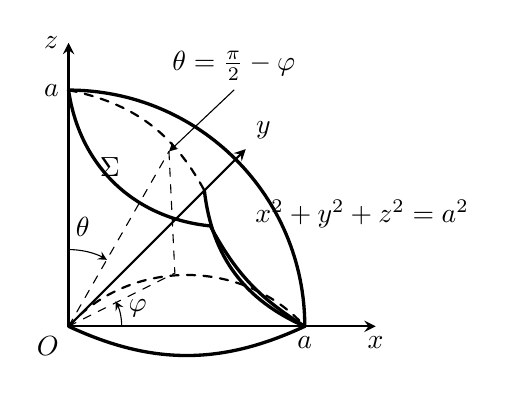
\begin{tikzpicture}[scale=1.5, >=stealth, line cap=round, line join=round]
    % 原点
    \coordinate (O) at (0,0);
    \node[below left] at (O) {$O$};
    
    % 坐标轴
    % z 轴向上
    \draw[->, thick] (0,0) -- (0,2.4) node[left] {$z$};
    % x 轴向右
    \draw[->, thick] (0,0) -- (2.6,0) node[below] {$x$};
    % y 轴向斜右上 (约 45 度)
    \draw[->, thick] (0,0) -- (1.5,1.5) node[above right] {$y$};
    
    % 球面在第一卦限的大圆轮廓
    % xOz 平面内圆弧 (半径 a = 2.0)
    \draw[very thick] (2.0,0) arc (0:90:2.0);
    \node[left] at (0,2.0) {$a$};
    \node[below] at (2.0,0) {$a$};
    
    % yOz 平面内的球面大圆弧 (虚线透视)
    \draw[dashed, thick] (0,2.0) to[bend left=25] (1.15,1.15);
    
    % xOy 平面内赤道大圆弧
    \draw[very thick] (2.0,0) to[bend left=30] (1.15,1.15);
    
    % 底面上柱面 x^2+y^2=ax 的半圆弧 (以 (1.0, 0) 为圆心，半径 1.0)
    \draw[dashed, thick] (0,0) to[bend left=48] (2.0,0);
    \draw[very thick] (0,0) to[bend right=25] (2.0,0);
    
    % 空间交线曲线: 球面与圆柱面交线 (在第一卦限的马鞍形空间拱线)
    % 从 (0,a) 到 (a,0) 弯曲
    \draw[very thick] (0,2.0) to[bend right=38] (1.2,0.85) to[bend right=15] (2.0,0);
    
    % 空间截面曲面片 Sigma 标注
    \node at (0.35,1.35) {$\Sigma$};
    
    % 球坐标辅助线与夹角 theta, phi:
    % 柱面上某一对应点 P
    \coordinate (P) at (0.85, 1.48);
    \coordinate (Pbot) at (0.90, 0.45);
    \draw[dashed] (P) -- (Pbot);
    \draw[dashed] (O) -- (P);
    \draw[dashed] (O) -- (Pbot);
    
    % 夹角 phi (在底面)
    \draw[->] (0.45,0) arc (0:28:0.45);
    \node[above right=-1pt] at (0.45,0.02) {$\varphi$};
    
    % 夹角 theta (与 z 轴夹角)
    \draw[->] (0,0.65) arc (90:60:0.65);
    \node[above] at (0.12,0.68) {$\theta$};
    
    % 方程指引关系
    \draw[<-] (P) -- (1.4, 2.0) node[above] {$\theta = \frac{\pi}{2} - \varphi$};
    \node[right] at (1.5, 0.95) {$x^{2}+y^{2}+z^{2}=a^{2}$};
  \end{tikzpicture}
  \caption{}\label{fig:11.1.7}
\end{figure}

\begin{example}\label{ex:11.1.6}
计算环面 $\Sigma: \boldsymbol{x}(\theta, \varphi)=((b+a \cos \theta) \cos \varphi,(b+a \cos \theta) \sin \varphi, a \sin \theta)$, $0 \leqslant \theta, \varphi \leqslant 2 \pi\ (0<a<b)$ 的表面积 $\sigma(\Sigma)$ (\cref{fig:11.1.8}).
\end{example}

\begin{solution}
\[
  \boldsymbol{x}_{\theta}^{\prime}=\left(-a \sin \theta \cos \varphi,-a \sin \theta \sin \varphi, a \cos \theta\right),
\]
\[
  \boldsymbol{x}_{\varphi}^{\prime}=\left(-(b+a \cos \theta) \sin \varphi,(b+a \cos \theta) \cos \varphi, 0\right),
\]
\[
  E=\boldsymbol{x}_{\theta}^{\prime} \cdot \boldsymbol{x}_{\theta}^{\prime}=a^{2}, \quad F=\boldsymbol{x}_{\theta}^{\prime} \cdot \boldsymbol{x}_{\varphi}^{\prime}=0\ \left(\boldsymbol{x}_{\theta}^{\prime} \perp \boldsymbol{x}_{\varphi}^{\prime}\right),
\]
\[
  G=\boldsymbol{x}_{\varphi}^{\prime} \cdot \boldsymbol{x}_{\varphi}^{\prime}=(b+a \cos \theta)^{2}.
\]
由此得到
\begin{align*}
  \sigma(\Sigma) &=\iint_{\substack{0 \leqslant \theta \leqslant 2 \pi \\ 0 \leqslant \varphi \leqslant 2 \pi}} \sqrt{E G-F^{2}}\,\mathrm{d} \theta \mathrm{d} \varphi \\
  &=\int_{0}^{2 \pi} \mathrm{d} \varphi \int_{0}^{2 \pi} a(b+a \cos \theta)\,\mathrm{d} \theta=2 \pi a\left(2 \pi b+a \sin \theta\bigg|_{0} ^{2 \pi}\right) \\
  &=4 \pi^{2} a b. \qedhere
\end{align*}
\end{solution}

\begin{figure}[htbp]
  \centering
  \begin{tikzpicture}[scale=1.45, >=stealth, line cap=round, line join=round]
    % 坐标轴
    \draw[->, thick] (-0.8,0) -- (3.6,0) node[below] {$x$};
    \draw[->, thick] (0,-1.5) -- (0,1.8) node[left] {$y$};
    \node[below left] at (0,0) {$O$};
    
    % 生成圆: 中心在 (b,0)，半径为 a (取 b=2.0, a=0.95)
    \coordinate (C) at (2.0,0);
    \draw[very thick] (C) circle (0.95);
    \node[below] at (2.0,0) {$b$};
    
    % 半径线段与角度 theta
    \coordinate (P) at ($(C) + (48:0.95)$);
    \draw[very thick] (C) -- (P);
    
    % 半径长 a 标注
    \node[above left] at ($(C)!0.55!(P)$) {$a$};
    
    % 夹角 theta
    \draw[->] (2.35,0) arc (0:48:0.35);
    \node[right] at (2.35,0.15) {$\theta$};
    
    % 圆方程标注
    \node[above right] at (1.65,0.98) {$(x-b)^{2}+y^{2}=a^{2}$};
  \end{tikzpicture}
  \caption{}\label{fig:11.1.8}
\end{figure}

\begin{example}\label{ex:11.1.7}
计算摆线一拱 $(x, y)=(a(t-\sin t), a(1-\cos t)), 0 \leqslant t \leqslant 2 \pi$ 绕 $x$ 轴旋转一周所得曲面 $\Sigma$ 的面积 $\sigma(\Sigma)$ (见第一册\extref{图 6.6.4}).
\end{example}

\begin{solution}[解法 1]
设摆线一拱为 $C$, 则
\begin{align*}
  \sigma(\Sigma) &=\int_{C} 2 \pi y\,\mathrm{d} s=2 \pi \int_{0}^{2 \pi} a(1-\cos t) \sqrt{\left[x^{\prime}(t)\right]^{2}+\left[y^{\prime}(t)\right]^{2}}\,\mathrm{d} t \\
  &=2 \pi a \int_{0}^{2 \pi}(1-\cos t) \sqrt{a^{2}(1-\cos t)^{2}+a^{2} \sin ^{2} t}\,\mathrm{d} t \\
  &=2 \pi a^{2} \int_{0}^{2 \pi}(1-\cos t) \sqrt{2(1-\cos t)}\,\mathrm{d} t=8 \pi a^{2} \int_{0}^{2 \pi} \sin ^{3} \frac{t}{2}\,\mathrm{d} t \\
  &=16 \pi a^{2} \int_{0}^{2 \pi}\left(\cos ^{2} \frac{t}{2}-1\right) \mathrm{d} \cos \frac{t}{2}=16 \pi a^{2}\left(\frac{\cos ^{3} \frac{t}{2}}{3}-\cos \frac{t}{2}\right)\bigg|_{0} ^{2 \pi}=\frac{64}{3} \pi a^{2}. \qedhere
\end{align*}
\end{solution}

\begin{solution}[解法 2]
旋转曲面 $\Sigma$ 的参数表示为
\begin{align*}
  \boldsymbol{x}(t, \varphi) &=(x(t, \varphi), y(t, \varphi), z(t, \varphi)) \\
  &=(a(t-\sin t), a(1-\cos t) \cos \varphi, a(1-\cos t) \sin \varphi), \\
  &\quad 0 \leqslant t \leqslant 2 \pi, \quad 0 \leqslant \varphi \leqslant 2 \pi.
\end{align*}
\[
  \boldsymbol{x}_{t}^{\prime}=(a(1-\cos t), a \sin t \cos \varphi, a \sin t \sin \varphi),
\]
\[
  \boldsymbol{x}_{\varphi}^{\prime}=(0,-a(1-\cos t) \sin \varphi, a(1-\cos t) \cos \varphi).
\]
\[
  E=\boldsymbol{x}_{t}^{\prime} \cdot \boldsymbol{x}_{t}^{\prime}=a^{2}\left[(1-\cos t)^{2}+\sin ^{2} t\right]=2 a^{2}(1-\cos t),
\]
\[
  F=\boldsymbol{x}_{t}^{\prime} \cdot \boldsymbol{x}_{\varphi}^{\prime}=0 \quad\left(\boldsymbol{x}_{t}^{\prime} \perp \boldsymbol{x}_{\varphi}^{\prime}\right).
\]
\[
  G=\boldsymbol{x}_{\varphi}^{\prime} \cdot \boldsymbol{x}_{\varphi}^{\prime}=a^{2}(1-\cos t)^{2}.
\]
\begin{align*}
  \sigma(\Sigma) &=\iint_{\substack{0 \leqslant t \leqslant 2 \pi \\ 0 \leqslant \varphi \leqslant 2 \pi}} \sqrt{E G-F^{2}}\,\mathrm{d} t \mathrm{d} \varphi=\iint_{\substack{0 \leqslant t \leqslant 2 \pi \\ 0 \leqslant \varphi \leqslant 2 \pi}} \sqrt{2} a^{2} \sqrt{(1-\cos t)^{3}}\,\mathrm{d} t \mathrm{d} \varphi \\
  &=4 a^{2} \int_{0}^{2 \pi} \sin ^{3} \frac{t}{2}\,\mathrm{d} t \int_{0}^{2 \pi} \mathrm{d} \varphi=8 \pi a^{2} \int_{0}^{2 \pi} \sin ^{3} \frac{t}{2}\,\mathrm{d} t=\frac{64}{3} \pi a^{2}. \qedhere
\end{align*}
\end{solution}

\begin{example}\label{ex:11.1.8}
将抛物线 $C: y=\sqrt{x}, 0 \leqslant x \leqslant a$ 绕 $x$ 轴旋转一周得旋转抛物面 $\Sigma$, 求它的面积 $\sigma(\Sigma)$.
\end{example}

\begin{solution}[解法 1]
\begin{align*}
  \sigma(\Sigma) &=\int_{C} 2 \pi y\,\mathrm{d} s=2 \pi \int_{0}^{a} \sqrt{x} \sqrt{1+\left[y^{\prime}(x)\right]^{2}}\,\mathrm{d} x \\
  &=2 \pi \int_{0}^{a} \sqrt{x} \sqrt{1+\frac{1}{4 x}}\,\mathrm{d} x=2 \pi \int_{0}^{a} \sqrt{x+\frac{1}{4}}\,\mathrm{d} x \\
  &=2 \pi \cdot \frac{2}{3}\left(x+\frac{1}{4}\right)^{\frac{3}{2}}\bigg|_{0} ^{a}=\frac{4 \pi}{3}\left[\left(a+\frac{1}{4}\right)^{\frac{3}{2}}-\frac{1}{8}\right] \\
  &=\frac{\pi}{6}\left[(4 a+1)^{\frac{3}{2}}-1\right]. \qedhere
\end{align*}
\end{solution}

\begin{solution}[解法 2]
旋转抛物面的参数表示为
\[
  \boldsymbol{x}(x, \varphi)=\left(x, \sqrt{x} \cos \varphi, \sqrt{x} \sin \varphi\right), \quad 0 \leqslant x \leqslant a,\ 0 \leqslant \varphi \leqslant 2 \pi.
\]
\[
  \boldsymbol{x}_{x}^{\prime}=\left(1, \frac{1}{2 \sqrt{x}} \cos \varphi, \frac{1}{2 \sqrt{x}} \sin \varphi\right),
\]
\[
  \boldsymbol{x}_{\varphi}^{\prime}=(0,-\sqrt{x} \sin \varphi, \sqrt{x} \cos \varphi).
\]
\[
  E=\boldsymbol{x}_{x}^{\prime} \cdot \boldsymbol{x}_{x}^{\prime}=1+\frac{1}{4 x},
\]
\[
  F=\boldsymbol{x}_{x}^{\prime} \cdot \boldsymbol{x}_{\varphi}^{\prime}=0 \quad\left(\boldsymbol{x}_{x}^{\prime} \perp \boldsymbol{x}_{\varphi}^{\prime}\right),
\]
\[
  G=\boldsymbol{x}_{\varphi}^{\prime} \cdot \boldsymbol{x}_{\varphi}^{\prime}=x.
\]
\begin{align*}
  \sigma(\Sigma) &=\iint_{\substack{0 \leqslant x \leqslant a \\ 0 \leqslant \varphi \leqslant 2 \pi}} \sqrt{E G-F^{2}}\,\mathrm{d} x \mathrm{d} \varphi=\iint_{\substack{0 \leqslant x \leqslant a \\ 0 \leqslant \varphi \leqslant 2 \pi}} \sqrt{x+\frac{1}{4}}\,\mathrm{d} x \mathrm{d} \varphi \\
  &=\int_{0}^{2 \pi} \mathrm{d} \varphi \int_{0}^{a} \sqrt{x+\frac{1}{4}}\,\mathrm{d} x \reason{由解法 1} \frac{\pi}{6}\left[(4 a+1)^{\frac{3}{2}}-1\right]. \qedhere
\end{align*}
\end{solution}

下面考虑一般的旋转曲面.

\begin{example}\label{ex:11.1.9}
将 $x O y$ 平面上的曲线 $C:(x, y)=(x(t), y(t)), \alpha \leqslant t \leqslant \beta$ 绕 $x$ 轴旋转一周得旋转曲面 $\Sigma$, 其中 $x(t), y(t)$ 都为 $C^{1}$ 函数. 求它的面积 $\sigma(\Sigma)$.
\end{example}

\begin{solution}[解法 1]
\[
  \sigma(\Sigma)=\int_{C} 2 \pi y\,\mathrm{d} s=2 \pi \int_{\alpha}^{\beta} y(t) \sqrt{\left[x^{\prime}(t)\right]^{2}+\left[y^{\prime}(t)\right]^{2}}\,\mathrm{d} t. \qedhere
\]
\end{solution}

\begin{solution}[解法 2]
旋转曲面 $\Sigma$ 的参数表示为
\[
  \boldsymbol{x}(t, \varphi)=(x(t), y(t) \cos \varphi, y(t) \sin \varphi), \quad \alpha \leqslant t \leqslant \beta,\ 0 \leqslant \varphi \leqslant 2 \pi.
\]
\[
  \boldsymbol{x}_{t}^{\prime}=\left(x^{\prime}(t), y^{\prime}(t) \cos \varphi, y^{\prime}(t) \sin \varphi\right),
\]
\[
  \boldsymbol{x}_{\varphi}^{\prime}=(0,-y(t) \sin \varphi, y(t) \cos \varphi).
\]
\[
  E=\boldsymbol{x}_{t}^{\prime} \cdot \boldsymbol{x}_{t}^{\prime}=\left[x^{\prime}(t)\right]^{2}+\left[y^{\prime}(t)\right]^{2},
\]
\[
  F=\boldsymbol{x}_{t}^{\prime} \cdot \boldsymbol{x}_{\varphi}^{\prime}=0 \quad\left(\boldsymbol{x}_{t}^{\prime} \perp \boldsymbol{x}_{\varphi}^{\prime}\right),
\]
\[
  G=\boldsymbol{x}_{\varphi}^{\prime} \cdot \boldsymbol{x}_{\varphi}^{\prime}=y^{2}(t).
\]
\begin{align*}
  \sigma(\Sigma) &=\iint_{\substack{\alpha \leqslant t \leqslant \beta \\ 0 \leqslant \varphi \leqslant 2 \pi}} \sqrt{E G-F^{2}}\,\mathrm{d} t \mathrm{d} \varphi=\iint_{\substack{\alpha \leqslant t \leqslant \beta \\ 0 \leqslant \varphi \leqslant 2 \pi}} y(t) \sqrt{\left[x^{\prime}(t)\right]^{2}+\left[y^{\prime}(t)\right]^{2}}\,\mathrm{d} t \mathrm{d} \varphi \\
  &=\int_{0}^{2 \pi} \mathrm{d} \varphi \int_{\alpha}^{\beta} y(t) \sqrt{\left[x^{\prime}(t)\right]^{2}+\left[y^{\prime}(t)\right]^{2}}\,\mathrm{d} t=2 \pi \int_{\alpha}^{\beta} y(t) \sqrt{\left[x^{\prime}(t)\right]^{2}+\left[y^{\prime}(t)\right]^{2}}\,\mathrm{d} t. \qedhere
\end{align*}
\end{solution}

\begin{example}\label{ex:11.1.10}
计算 $\mathbb{R}^{n}$ 中以原点为中心 $a>0$ 为半径的 $n-1$ 维球面 $S^{n-1}(a)$ 的面积 $\sigma\left(S^{n-1}(a)\right)$.
\end{example}

\begin{solution}[解法 1]
应用 $n-1$ 维球面坐标变换
\[
  \left\{\begin{aligned}
    x_{1} &=a \cos \theta_{1}, \\
    x_{2} &=a \sin \theta_{1} \cos \theta_{2}, \\
    x_{3} &=a \sin \theta_{1} \sin \theta_{2} \cos \theta_{3}, \\
    & \vdots \\
    x_{n-1} &=a \sin \theta_{1} \sin \theta_{2} \sin \theta_{3} \cdots \sin \theta_{n-2} \cos \theta_{n-1}, \\
    x_{n} &=a \sin \theta_{1} \sin \theta_{2} \sin \theta_{3} \cdots \sin \theta_{n-2} \sin \theta_{n-1},
  \end{aligned}\right.
\]
\[
  0 \leqslant \theta_{1}, \theta_{2}, \cdots, \theta_{n-2} \leqslant \pi, \quad 0 \leqslant \theta_{n-1} \leqslant 2 \pi.
\]
读者可以证明 $n-1$ 维球面 $S^{n-1}(a)$ 的面积元为 (复习题 11 题 2)
\begin{align*}
  \mathrm{d} \sigma &=\sqrt{\operatorname{det}\begin{pmatrix}
      g_{11} & \cdots & g_{1, n-1} \\
      \vdots & & \vdots \\
      g_{n-1,1} & \cdots & g_{n-1, n-1}
    \end{pmatrix}}\,\mathrm{d} \theta_{1} \mathrm{d} \theta_{2} \cdots \mathrm{d} \theta_{n-1} \\
  &=a^{n-1} \sin ^{n-2} \theta_{1} \sin ^{n-3} \theta_{2} \cdots \sin \theta_{n-2}\,\mathrm{d} \theta_{1} \mathrm{d} \theta_{2} \cdots \mathrm{d} \theta_{n-1}.
\end{align*}
因此, $S^{n-1}(a)$ 的面积为
\begin{align*}
  \sigma\left(S^{n-1}(a)\right) &=\int_{\substack{0 \leqslant \theta_{1}, \theta_{2}, \cdots, \theta_{n-2} \leqslant \pi \\ 0 \leqslant \theta_{n-1} \leqslant 2 \pi}} a^{n-1} \sin ^{n-2} \theta_{1} \sin ^{n-3} \theta_{2} \cdots \sin \theta_{n-2}\,\mathrm{d} \theta_{1} \cdots \mathrm{d} \theta_{n-1} \\
  &=a^{n-1} \cdot n \int_{0}^{1} r^{n-1}\,\mathrm{d} r \int_{\substack{0 \leqslant \theta_{1}, \theta_{2}, \cdots, \theta_{n-2} \leqslant \pi \\ 0 \leqslant \theta_{n-1} \leqslant 2 \pi}} \sin ^{n-2} \theta_{1} \sin ^{n-3} \theta_{2} \cdots \sin \theta_{n-2}\,\mathrm{d} \theta_{1} \cdots \mathrm{d} \theta_{n-1} \\
  &=n a^{n-1} v\left(B_{n}(1)\right)=\left\{\begin{aligned}
      &2 k a^{2 k-1} \cdot \frac{\pi^{k}}{k!}, & & n=2 k, \\
      &(2 k-1) a^{2 k-2} \cdot \frac{2^{k} \pi^{k-1}}{(2 k-1)!!}, & & n=2 k-1
    \end{aligned}\right. \\
  &=\left\{\begin{aligned}
      &\frac{2 \pi^{k}}{(k-1)!} a^{2 k-1}, & & n=2 k, \\
      &\frac{2^{k} \pi^{k-1}}{(2 k-3)!!} a^{2 k-2}, & & n=2 k-1
    \end{aligned}\right. \\
  &=\frac{2 \pi^{\frac{n}{2}}}{\Gamma\left(\frac{n}{2}\right)} a^{n-1}. \qedhere
\end{align*}
\end{solution}

\begin{solution}[解法 2]
因为 $x_{1}^{2}+x_{2}^{2}+\cdots+x_{n}^{2}=a^{2},\ 2 x_{i}+2 x_{n} \cdot \frac{\partial x_{n}}{\partial x_{i}}=0$, 即
\[
  \frac{\partial x_{n}}{\partial x_{i}}=-\frac{x_{i}}{x_{n}}.
\]
所以 $S^{n-1}(a)$ 的上半球面可由方程
\[
  x_{n}=\sqrt{a^{2}-\left(x_{1}^{2}+x_{2}^{2}+\cdots+x_{n-1}^{2}\right)}, \quad x_{1}^{2}+x_{2}^{2}+\cdots+x_{n-1}^{2} \leqslant a^{2}
\]
确定. 于是,
\begin{align*}
  \sigma\left(S^{n-1}(a)\right) &=2 \idotsint_{x_{1}^{2}+x_{2}^{2}+\cdots+x_{n-1}^{2} \leqslant a^{2}} \sqrt{1+\left(\frac{\partial x_{n}}{\partial x_{1}}\right)^{2}+\cdots+\left(\frac{\partial x_{n}}{\partial x_{n-1}}\right)^{2}}\,\mathrm{d} x_{1} \cdots \mathrm{d} x_{n-1} \\
  &=2 \idotsint_{x_{1}^{2}+\cdots+x_{n-1}^{2} \leqslant a^{2}} \sqrt{1+\left(-\frac{x_{1}}{x_{n}}\right)^{2}+\cdots+\left(-\frac{x_{n-1}}{x_{n}}\right)^{2}}\,\mathrm{d} x_{1} \cdots \mathrm{d} x_{n-1} \\
  &=2 \idotsint_{x_{1}^{2}+\cdots+x_{n-1}^{2} \leqslant a^{2}} \frac{a}{x_{n}}\,\mathrm{d} x_{1} \cdots \mathrm{d} x_{n-1} \\
  &\reasonb{\extref{例 10.5.14}} {x_{i}=a y_{i},\ i=1,2, \cdots, n-1} 2 \idotsint_{y_{1}^{2}+\cdots+y_{n-1}^{2} \leqslant 1} \\
  &\quad \frac{a}{\sqrt{a^{2}-a^{2}\left(y_{1}^{2}+\cdots+y_{n-1}^{2}\right)}}\, a^{n-1}\,\mathrm{d} y_{1} \cdots \mathrm{d} y_{n-1} \\
  &=2 a^{n-1} \idotsint_{y_{1}^{2}+\cdots+y_{n-1}^{2} \leqslant 1} \frac{\mathrm{d} y_{1} \cdots \mathrm{d} y_{n-1}}{\sqrt{1-\left(y_{1}^{2}+\cdots+y_{n-1}^{2}\right)}}=a^{n-1} \sigma\left(S^{n-1}(1)\right) \\
  &\reason{\extref{例 10.5.14}}\left\{\begin{aligned}
      &\frac{2 \pi^{k}}{(k-1)!} a^{2 k-1}, & & n=2 k, \\
      &\frac{2^{k} \pi^{k-1}}{(2 k-3)!!} a^{2 k-2}, & & n=2 k-1
    \end{aligned}\right. \\
  &=\frac{2 \pi^{\frac{n}{2}}}{\Gamma\left(\frac{n}{2}\right)} a^{n-1}. \qedhere
\end{align*}
\end{solution}

\begin{example}\label{ex:11.1.11}
设 $\Sigma$ 为锥面 $z^{2}=k^{2}\left(x^{2}+y^{2}\right)(k>0)$ 被柱面 $x^{2}+y^{2}=2 a x$ 截下的部分. 计算曲面积分
\[
  \iint_{\Sigma}\left(y^{2} z^{2}+z^{2} x^{2}+x^{2} y^{2}\right) \mathrm{d} \sigma.
\]
\end{example}

\begin{solution}
设 $\Sigma$ 的上半部为
\[
  z=k \sqrt{x^{2}+y^{2}}, \quad x^{2}+y^{2} \leqslant 2 a x, \quad z>0,
\]
故面积元为
\[
  \mathrm{d} \sigma=\sqrt{1+\left(\frac{\partial z}{\partial x}\right)^{2}+\left(\frac{\partial z}{\partial y}\right)^{2}}\,\mathrm{d} x \mathrm{d} y=\sqrt{1+\frac{k^{2} x^{2}}{x^{2}+y^{2}}+\frac{k^{2} y^{2}}{x^{2}+y^{2}}}\,\mathrm{d} x \mathrm{d} y=\sqrt{1+k^{2}}\,\mathrm{d} x \mathrm{d} y.
\]
\begin{align*}
  \iint_{\Sigma} & \left(y^{2} z^{2}+z^{2} x^{2}+x^{2} y^{2}\right) \mathrm{d} \sigma \\
  &\reason{对称性} 4 \iint_{\substack{x^{2}+y^{2} \leqslant 2 a x \\ x, y \geqslant 0}}\left[\left(x^{2}+y^{2}\right) k^{2}\left(x^{2}+y^{2}\right)+x^{2} y^{2}\right] \sqrt{1+k^{2}}\,\mathrm{d} x \mathrm{d} y \\
  &=4 \sqrt{1+k^{2}} \iint_{\substack{x^{2}+y^{2} \leqslant 2 a x \\ x, y \geqslant 0}}\left[k^{2}\left(x^{2}+y^{2}\right)^{2}+x^{2} y^{2}\right] \mathrm{d} x \mathrm{d} y \\
  &\reason{极坐标变换} 4 \sqrt{1+k^{2}} \int_{0}^{\frac{\pi}{2}} \mathrm{d} \varphi \int_{0}^{2 a \cos \varphi}\left[k^{2} r^{4}+r^{4} \sin ^{2} \varphi \cos ^{2} \varphi\right] r\,\mathrm{d} r \\
  &=4 \sqrt{1+k^{2}} \int_{0}^{\frac{\pi}{2}}\left(k^{2}+\sin ^{2} \varphi \cos ^{2} \varphi\right) \frac{r^{6}}{6}\bigg|_{0} ^{2 a \cos \varphi} \mathrm{d} \varphi \\
  &=\frac{128 a^{6}}{3} \sqrt{1+k^{2}} \int_{0}^{\frac{\pi}{2}}\left(k^{2}+\sin ^{2} \varphi \cos ^{2} \varphi\right) \cos ^{6} \varphi\,\mathrm{d} \varphi \\
  &=\frac{128 a^{6}}{3} \sqrt{1+k^{2}} \int_{0}^{\frac{\pi}{2}}\left(k^{2} \cos ^{6} \varphi+\cos ^{8} \varphi-\cos ^{10} \varphi\right) \mathrm{d} \varphi \\
  &=\frac{128 a^{6}}{3} \sqrt{1+k^{2}}\left(k^{2} \cdot \frac{5 \times 3}{6 \times 4 \times 2}+\frac{7 \times 5 \times 3}{8 \times 6 \times 4 \times 2}-\frac{9 \times 7 \times 5 \times 3}{10 \times 8 \times 6 \times 4 \times 2}\right) \frac{\pi}{2} \\
  &=\frac{128 a^{6}}{3} \sqrt{1+k^{2}} \cdot \frac{5}{16}\left(k^{2}+\frac{7}{8}-\frac{63}{80}\right) \cdot \frac{\pi}{2}=\frac{\pi}{12}\left(80 k^{2}+7\right) \sqrt{1+k^{2}} a^{6}. \qedhere
\end{align*}
\end{solution}

\begin{example}\label{ex:11.1.12}
设 $\Sigma=\left\{(x, y, z) \mid x^{2}+y^{2}=a^{2},\ 0 \leqslant z \leqslant h\right\}$ 为圆柱面. 计算第一型曲面积分
\[
  \iint_{\Sigma}\left(x^{4}+y^{4}\right) \mathrm{d} \sigma.
\]
\end{example}

\begin{solution}
由于 $\Sigma$ 为圆柱面, 故采用柱面坐标变换
\[
  \boldsymbol{x}(\varphi, z)=(x, y, z)=(a \cos \varphi, a \sin \varphi, z).
\]
于是,
\[
  \boldsymbol{x}_{\varphi}^{\prime}=(-a \sin \varphi, a \cos \varphi, 0),
\]
\[
  \boldsymbol{x}_{z}^{\prime}=(0,0,1),
\]
\[
  E=\boldsymbol{x}_{\varphi}^{\prime} \cdot \boldsymbol{x}_{\varphi}^{\prime}=a^{2}, \quad F=\boldsymbol{x}_{\varphi}^{\prime} \cdot \boldsymbol{x}_{z}^{\prime}=0 \quad\left(\boldsymbol{x}_{\varphi}^{\prime} \perp \boldsymbol{x}_{z}^{\prime}\right), \quad G=\boldsymbol{x}_{z}^{\prime} \cdot \boldsymbol{x}_{z}^{\prime}=1.
\]
面积元为 $\mathrm{d} \sigma=\sqrt{E G-F^{2}}\,\mathrm{d} \varphi \mathrm{d} z=a\,\mathrm{d} \varphi \mathrm{d} z$. 从而第一型曲面积分
\begin{align*}
  \iint_{\Sigma} & \left(x^{4}+y^{4}\right) \mathrm{d} \sigma \reason{对称性} 2 \iint_{\Sigma} y^{4}\,\mathrm{d} \sigma \reason{柱面坐标变换} 2 \iint_{\substack{0 \leqslant \varphi \leqslant 2 \pi \\ 0 \leqslant z \leqslant h}} a^{4} \sin ^{4} \varphi \cdot a\,\mathrm{d} \varphi \mathrm{d} z \\
  &=8 a^{5} \int_{0}^{\frac{\pi}{2}} \sin ^{4} \varphi\,\mathrm{d} \varphi \cdot \int_{0}^{h} \mathrm{d} z=8 a^{5} h \cdot \frac{3 \cdot 1}{4 \cdot 2} \cdot \frac{\pi}{2}=\frac{3}{2} \pi h a^{5}. \qedhere
\end{align*}
\end{solution}

\begin{example}\label{ex:11.1.13}
设 $\Sigma=\left\{(x, y, z) \mid x^{2}+y^{2}+z^{2}=a^{2},\ z \geqslant 0\right\}$ 为半球面. 计算第一型曲面积分
\[
  \iint_{\Sigma}(x+y+z)\,\mathrm{d} \sigma.
\]
\end{example}

\begin{solution}
因为 $\int_{\Sigma} x\,\mathrm{d} \sigma \reason{$x$ 为奇函数} 0$, $\int_{\Sigma} y\,\mathrm{d} \sigma \reason{$y$ 为奇函数} 0$, 故
\begin{align*}
  \iint_{\Sigma}(x+y+z)\,\mathrm{d} \sigma &=\iint_{\Sigma} z\,\mathrm{d} \sigma=\iint_{x^{2}+y^{2} \leqslant a^{2}} z \sqrt{1+\left(\frac{\partial z}{\partial x}\right)^{2}+\left(\frac{\partial z}{\partial y}\right)^{2}}\,\mathrm{d} x \mathrm{d} y \\
  &=\iint_{x^{2}+y^{2} \leqslant a^{2}} z \sqrt{1+\left(-\frac{x}{z}\right)^{2}+\left(-\frac{y}{z}\right)^{2}}\,\mathrm{d} x \mathrm{d} y=\iint_{x^{2}+y^{2} \leqslant a^{2}} z \cdot \frac{a}{z}\,\mathrm{d} x \mathrm{d} y \\
  &=a \cdot \pi a^{2}=\pi a^{3}. \qedhere
\end{align*}
\end{solution}

\begin{example}\label{ex:11.1.14}
设 $S^{2}(a)$ 是以原点为中心 $a$ 为半径的球面, 即 $x^{2}+y^{2}+z^{2}=a^{2}$. 计算第一型曲面积分 $\iint_{S^{2}(a)} x^{2}\,\mathrm{d} \sigma$.
\end{example}

\begin{solution}[解法 1]
应用球面坐标, 有
\begin{align*}
  \iint_{S^{2}(a)} x^{2}\,\mathrm{d} \sigma &=\iint_{\substack{0 \leqslant \varphi \leqslant 2 \pi \\ 0 \leqslant \theta \leqslant \pi}} a^{2} \sin ^{2} \theta \cos ^{2} \varphi \cdot a^{2} \sin \theta\,\mathrm{d} \theta \mathrm{d} \varphi \\
  &=a^{4} \int_{0}^{2 \pi} \cos ^{2} \varphi\,\mathrm{d} \varphi \int_{0}^{\pi} \sin ^{3} \theta\,\mathrm{d} \theta=8 a^{4} \int_{0}^{\frac{\pi}{2}} \cos ^{2} \varphi\,\mathrm{d} \varphi \int_{0}^{\frac{\pi}{2}} \sin ^{3} \theta\,\mathrm{d} \theta \\
  &=8 a^{4} \cdot \frac{\pi}{4} \cdot \frac{2}{3}=\frac{4}{3} \pi a^{4}. \qedhere
\end{align*}
\end{solution}

\begin{solution}[解法 2]
由对称性显然有
\[
  \iint_{S^{2}(a)} x^{2}\,\mathrm{d} \sigma=\iint_{S^{2}(a)} y^{2}\,\mathrm{d} \sigma=\iint_{S^{2}(a)} z^{2}\,\mathrm{d} \sigma.
\]
将上面三式相加得到
\begin{align*}
  \iint_{S^{2}(a)} x^{2}\,\mathrm{d} \sigma &=\frac{1}{3} \iint_{S^{2}(a)}\left(x^{2}+y^{2}+z^{2}\right) \mathrm{d} \sigma=\frac{a^{2}}{3} \iint_{S^{2}(a)} \mathrm{d} \sigma=\frac{a^{2}}{3} \sigma\left(S^{2}(a)\right) \\
  &=\frac{a^{2}}{3} \cdot 4 \pi a^{2}=\frac{4}{3} \pi a^{4}. \qedhere
\end{align*}
\end{solution}

\begin{example}\label{ex:11.1.15}
设 $\Sigma$ 是球面 $x^{2}+y^{2}+z^{2}=a^{2}$ 被平面 $z=h\ (0<h<a)$ 所截的顶部 (\cref{fig:11.1.9}), 计算第一型曲面积分 $\iint_{\Sigma} \frac{\mathrm{d} \sigma}{z}$.
\end{example}

\begin{solution}
曲面 $\Sigma$ 的参数表示为 $\boldsymbol{x}(x, y)=(x, y, z)=(x, y, \sqrt{a^{2}-x^{2}-y^{2}})$, 其中 $\Delta=\{(x, y) \mid x^{2}+y^{2} \leqslant a^{2}-h^{2}\}$. 由于面积元
\[
  \mathrm{d} \sigma=\sqrt{1+\left(z_{x}^{\prime}\right)^{2}+\left(z_{y}^{\prime}\right)^{2}}\,\mathrm{d} x \mathrm{d} y=\frac{a}{\sqrt{a^{2}-x^{2}-y^{2}}}\,\mathrm{d} x \mathrm{d} y,
\]
所以,
\begin{align*}
  \iint_{\Sigma} \frac{\mathrm{d} \sigma}{z} &=\iint_{\Delta} \frac{1}{\sqrt{a^{2}-x^{2}-y^{2}}} \cdot \frac{a}{\sqrt{a^{2}-x^{2}-y^{2}}}\,\mathrm{d} x \mathrm{d} y \\
  &\reason{极坐标变换} a \int_{0}^{2 \pi} \mathrm{d} \varphi \int_{0}^{\sqrt{a^{2}-h^{2}}} \frac{r}{a^{2}-r^{2}}\,\mathrm{d} r \\
  &=-\pi a \ln \left(a^{2}-r^{2}\right)\bigg|_{0} ^{\sqrt{a^{2}-h^{2}}}=\pi a\left(\ln a^{2}-\ln h^{2}\right) \\
  &=2 \pi a \ln \frac{a}{h}. \qedhere
\end{align*}
\end{solution}

\begin{figure}[htbp]
  \centering
  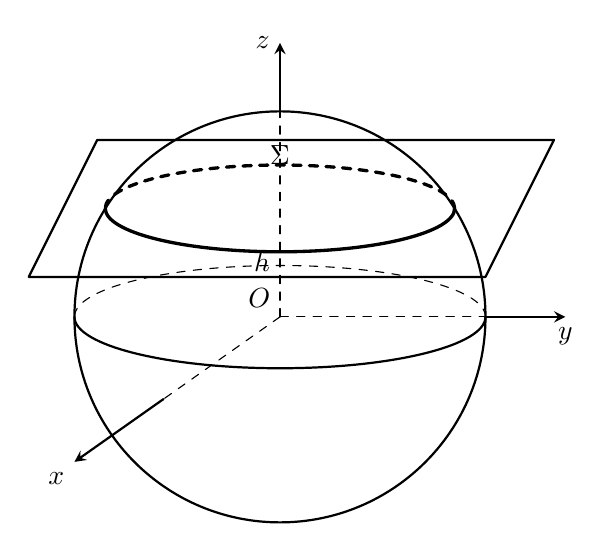
\begin{tikzpicture}[scale=1.45, >=stealth, line cap=round, line join=round]
    % 球面外轮廓圆
    \draw[thick] (0,0) circle (1.8);
    
    % 赤道椭圆: 后半虚线，前半实线
    \draw[dashed] (1.8,0) arc (0:180:1.8 and 0.45);
    \draw[thick] (-1.8,0) arc (180:360:1.8 and 0.45);
    
    % 坐标轴
    % z 轴
    \draw[dashed] (0,0) -- (0,1.8);
    \draw[->, thick] (0,1.8) -- (0,2.4) node[left] {$z$};
    
    % y 轴
    \draw[dashed] (0,0) -- (1.8,0);
    \draw[->, thick] (1.8,0) -- (2.5,0) node[below] {$y$};
    
    % x 轴 (左前约 215 度)
    \draw[dashed] (0,0) -- (-1.02,-0.72);
    \draw[->, thick] (-1.02,-0.72) -- (-1.8,-1.27) node[below left] {$x$};
    
    \node[above left] at (0,0) {$O$};
    
    % 水平截平面 z=h (高度 h = 0.95, 截圆半径 r = sqrt(1.8^2 - 0.95^2) = 1.53)
    % 切面板 (透视平行四边形)
    \draw[thick] (-2.2,0.95-0.6) -- (1.8,0.95-0.6) -- (2.4,0.95+0.6) -- (-1.6,0.95+0.6) -- cycle;
    
    % 截出的小圆 (截面椭圆: 后半虚线，前半实线)
    \draw[dashed, very thick] (1.53,0.95) arc (0:180:1.53 and 0.38);
    \draw[very thick] (-1.53,0.95) arc (180:360:1.53 and 0.38);
    
    % 截面高度 h 标注 (在 z 轴上)
    \node[left] at (0,0.48) {$h$};
    
    % 球冠截顶部分顶部标注 Sigma
    \node[above] at (0,1.25) {$\Sigma$};
  \end{tikzpicture}
  \caption{}\label{fig:11.1.9}
\end{figure}

\begin{example}\label{ex:11.1.16}
设 $\Sigma$ 为螺旋面 (\cref{fig:11.1.10}) 的一部分, 它的参数表示为
\begin{align*}
  \boldsymbol{x}(u, v) &=(x(u, v), y(u, v), z(u, v)) \\
  &=(u \cos v, u \sin v, v),
\end{align*}
\[
  (u, v) \in \Delta=[0, a] \times[0,2 \pi].
\]
计算第一型曲面积分 $\iint_{\Sigma} z\,\mathrm{d} \sigma$.
\end{example}

\begin{solution}
$\boldsymbol{x}_{u}^{\prime}=(\cos v, \sin v, 0)$,
\[
  \boldsymbol{x}_{v}^{\prime}=(-u \sin v, u \cos v, 1),
\]
\[
  E=\boldsymbol{x}_{u}^{\prime} \cdot \boldsymbol{x}_{u}^{\prime}=1,
\]
\[
  F=\boldsymbol{x}_{u}^{\prime} \cdot \boldsymbol{x}_{v}^{\prime}=0 \quad\left(\boldsymbol{x}_{u}^{\prime} \perp \boldsymbol{x}_{v}^{\prime}\right), \quad G=\boldsymbol{x}_{v}^{\prime} \cdot \boldsymbol{x}_{v}^{\prime}=1+u^{2}.
\]
于是,
\begin{align*}
  \iint_{\Sigma} z\,\mathrm{d} \sigma &=\iint_{\Delta} v \sqrt{E G-F^{2}}\,\mathrm{d} u \mathrm{d} v=\int_{0}^{a} \sqrt{1+u^{2}}\,\mathrm{d} u \int_{0}^{2 \pi} v\,\mathrm{d} v \\
  &=\left[\frac{u}{2} \sqrt{1+u^{2}}+\frac{1}{2} \ln \left(u+\sqrt{1+u^{2}}\right)\right]\bigg|_{0} ^{a} \cdot \frac{v^{2}}{2}\bigg|_{0} ^{2 \pi} \\
  &=\pi^{2}\left[a \sqrt{1+a^{2}}+\ln \left(a+\sqrt{1+a^{2}}\right)\right]. \qedhere
\end{align*}
\end{solution}

\begin{figure}[htbp]
  \centering
  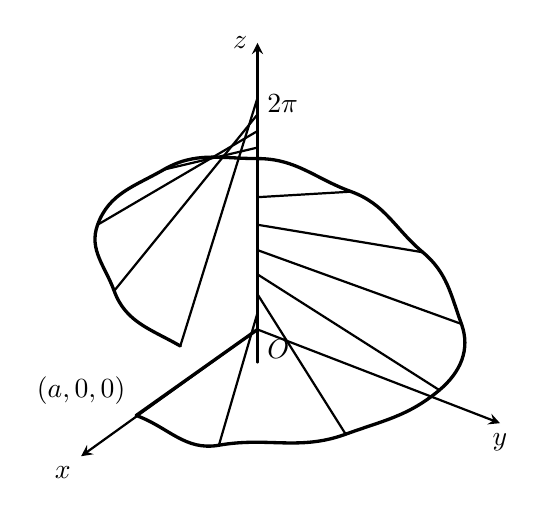
\begin{tikzpicture}[scale=1.4, >=stealth, line cap=round, line join=round]
    % 坐标轴
    % z 轴向上
    \draw[->, thick] (0,-0.3) -- (0,2.6) node[left] {$z$};
    % x 轴向左前 (约 215 度)
    \draw[->, thick] (0,0) -- (-1.6,-1.15) node[below left] {$x$};
    % y 轴向右下 (约 -30 度)
    \draw[->, thick] (0,0) -- (2.2,-0.85) node[below] {$y$};
    \node[below right] at (0,0) {$O$};
    
    % 螺旋面参数曲面片:
    % 从 x 轴上点 (a, 0, 0) 开始，绕 z 轴逆时针旋转上升一周 (0 <= v <= 2pi)
    % 辐射母线 (外端为螺旋线，内端在 z 轴)
    % 起点母线
    \coordinate (Start) at (-1.1,-0.78);
    \draw[very thick] (0,0) -- (Start) node[above left] {$(a,0,0)$};
    
    % 螺旋线上升轮廓 (用光滑贝塞尔曲线连接各母线外端点)
    % 采样辐射母线 (v = 0 到 360 度，对应 z 从 0 到 1.85)
    \coordinate (P0) at (-1.10, -0.78);
    \coordinate (P1) at (-0.35, -1.05);
    \coordinate (P2) at (0.80, -0.95);
    \coordinate (P3) at (1.65, -0.55);
    \coordinate (P4) at (1.85, 0.05);
    \coordinate (P5) at (1.50, 0.70);
    \coordinate (P6) at (0.85, 1.25);
    \coordinate (P7) at (0.00, 1.55);
    \coordinate (P8) at (-0.85, 1.45);
    \coordinate (P9) at (-1.45, 0.95);
    \coordinate (P10) at (-1.30, 0.35);
    \coordinate (P11) at (-0.70, -0.15);
    
    % 绘制辐射母线
    \draw[thick] (0,0.15) -- (P1);
    \draw[thick] (0,0.32) -- (P2);
    \draw[thick] (0,0.50) -- (P3);
    \draw[thick] (0,0.72) -- (P4);
    \draw[thick] (0,0.95) -- (P5);
    \draw[thick] (0,1.20) -- (P6);
    \draw[thick] (0,1.45) -- (P7);
    \draw[thick] (0,1.65) -- (P8);
    \draw[thick] (0,1.80) -- (P9);
    \draw[thick] (0,1.95) -- (P10);
    \draw[thick] (0,2.10) -- (P11);
    
    % 顶端母线与高度 2pi 标注
    \node[right] at (0,2.05) {$2\pi$};
    
    % 外边界螺旋线
    \draw[very thick] (P0) to[out=-20, in=190] (P1) to[out=10, in=200] (P2) to[out=20, in=220] (P3)
      to[out=40, in=-70] (P4) to[out=110, in=-40] (P5) to[out=140, in=-20] (P6)
      to[out=160, in=0] (P7) to[out=180, in=30] (P8) to[out=210, in=70] (P9)
      to[out=250, in=110] (P10) to[out=290, in=150] (P11);
      
    % 内轴线
    \draw[very thick] (0,0) -- (0,2.10);
  \end{tikzpicture}
  \caption{}\label{fig:11.1.10}
\end{figure}

\begin{exblock}{练习题 11.1}
\item 计算下列第一型曲线积分:
\begin{enumerate}[label=(\arabic*),leftmargin=2.6em,itemsep=0.15\baselineskip,topsep=0.2\baselineskip]
  \item $\int_{C}\left(x^{2}+y^{2}\right)^{n} \mathrm{d} s,\ C:\ (x, y)=(a \cos t, a \sin t),\ 0 \leqslant t \leqslant 2 \pi,\ n \in \mathbb{Z}_{+},\ a>0$;
  \item $\int_{C}(x+y)\,\mathrm{d} s,\ C$: 顶点为 $(0,0),(1,0),(0,1)$ 的三角形边界;
  \item $\int_{C} z\,\mathrm{d} s,\ C$: 圆锥螺线 $(x, y, z)=(t \cos t, t \sin t, t),\ t \in[0,2 \pi]$;
  \item $\int_{C} x^{2}\,\mathrm{d} s,\ C$: 圆周 $x^{2}+y^{2}+z^{2}=a^{2},\ x+y+z=0$;
  \item $\int_{C} z\,\mathrm{d} s,\ C:\ x^{2}+y^{2}=z^{2},\ y^{2}=a x$, 由 $(0,0,0)$ 到 $(a, a, \sqrt{2} a)$ 之间的一段, 其中 $a>0$;
  \item $\int_{C} y^{2}\,\mathrm{d} s,\ C$: 旋轮线的一拱, $(x, y)=(a(t-\sin t), a(1-\cos t)),\ 0 \leqslant t \leqslant 2 \pi$.
\end{enumerate}

\item 考察椭圆
\[
  \frac{x^{2}}{a^{2}}+\frac{y^{2}}{b^{2}}=1 \quad(a>b \geqslant 0),
\]
称
\[
  e=\sqrt{\frac{a^{2}-b^{2}}{a^{2}}}
\]
为该椭圆的离心率. 试通过 $e$ 和曲线积分来表示椭圆的周长.

\item 曲线 $C$ 用极坐标方程 $r=f(\varphi)(\alpha \leqslant \varphi \leqslant \beta)$ 所表示, 其中 $f$ 连续可导. 证明: $C$ 的长度为
\[
  \int_{\alpha}^{\beta} \sqrt{f^{2}(\varphi)+\left[f^{\prime}(\varphi)\right]^{2}}\,\mathrm{d} \varphi.
\]
利用这公式表达题 2 中椭圆的周长.

\item 计算下列曲面的面积:
\begin{enumerate}[label=(\arabic*),leftmargin=2.6em,itemsep=0.15\baselineskip,topsep=0.2\baselineskip]
  \item 锥面 $z=\sqrt{x^{2}+y^{2}}$ 被圆柱面 $x^{2}+y^{2}=2 x$ 截下的部分;
  \item 圆柱面 $x^{2}+z^{2}=a^{2}$ 被圆柱面 $x^{2}+y^{2}=a^{2}$ 截下的部分 $(a>0)$;
  \item 圆柱面介于平面 $x+z=0$ 与 $x-y=0$ 之间的部分;
  \item 球面 $x^{2}+y^{2}+z^{2}=a^{2}$ 被椭圆柱面
    \[
      \frac{x^{2}}{a^{2}}+\frac{y^{2}}{b^{2}}=1 \quad(0<b \leqslant a)
    \]
    所截下的部分;
  \item 马鞍面 $a z=x y$ 被圆柱面 $x^{2}+y^{2}=a^{2}$ 截下的部分 $(a>0)$;
  \item 抛物面 $x^{2}+y^{2}=2 a z$ 被柱面 $\left(x^{2}+y^{2}\right)^{2}=2 a^{2} x y$ 截下的部分 $(a>0)$;
  \item 螺旋面 $(x, y, z)=(r \cos \theta, r \sin \theta, h \theta),\ (r, \theta) \in(0, a) \times[0,2 \pi]$.
\end{enumerate}

\item 计算下列第一型曲面积分:
\begin{enumerate}[label=(\arabic*),leftmargin=2.6em,itemsep=0.15\baselineskip,topsep=0.2\baselineskip]
  \item $\iint_{\Sigma} \frac{\mathrm{d} \sigma}{(1+x+y)^{2}}$, 其中 $\Sigma$ 为四面体 $x+y+z \leqslant 1,\ x, y, z \geqslant 0$ 的边界;
  \item $\iint_{\Sigma}|x y z| \mathrm{d} \sigma,\ \Sigma:\ z=x^{2}+y^{2},\ z \leqslant 1$;
  \item $\iint_{\Sigma}(x y+y z+z x) \mathrm{d} \sigma,\ \Sigma:\ z=\sqrt{x^{2}+y^{2}}$ 被圆柱面 $x^{2}+y^{2}=2 x$ 割下的部分.
\end{enumerate}
\end{exblock}

\begin{exblock}{思考题 11.1}
\item 设 $\Sigma$ 为单位球面 $x^{2}+y^{2}+z^{2}=1$. 证明:
\[
  \iint_{\Sigma} f(a x+b y+c z)\,\mathrm{d} \sigma=2 \pi \int_{-1}^{1} f\left(\sqrt{a^{2}+b^{2}+c^{2}}\, t\right) \mathrm{d} t.
\]

\item 设 $\Sigma(t)$ 是平面 $x+y+z=t$ 被球面 $x^{2}+y^{2}+z^{2}=1$ 截下的部分, 且
\[
  F(x, y, z)=1-\left(x^{2}+y^{2}+z^{2}\right).
\]
证明: 对于 $|t| \leqslant \sqrt{3}$ 时, 有
\[
  \iint_{\Sigma(t)} F(x, y, z)\,\mathrm{d} \sigma=\frac{\pi}{18}\left(3-t^{2}\right).
\]

\item 对常数 $a>0$, 定义函数
\[
  f(x, y, z)=\left\{\begin{aligned}
    &1, & & x^{2}+y^{2}+z^{2} \leqslant a^{2}, \\
    &0, & & x^{2}+y^{2}+z^{2}>a^{2}.
  \end{aligned}\right.
\]
设 $\mathbb{R}^{3}$ 中的点 $(\xi, \eta, \zeta)$ 满足 $\xi^{2}+\eta^{2}+\zeta^{2}>a^{2}$, 计算第一型曲面积分
\[
  F(\xi, \eta, \zeta, t)=\iint_{\Sigma(t)} f(x, y, z)\,\mathrm{d} \sigma,
\]
其中 $\Sigma(t)$ 为球面 $(x-\xi)^{2}+(y-\eta)^{2}+(z-\zeta)^{2}=t^{2}$.

\item 设 $C$ 为右半 $y O z$ 平面中的 $C^{1}$ 简单曲线 $(y, z)=(\psi(u), \varphi(u)),\ a \leqslant u \leqslant b$. 让 $C$ 绕 $z$ 轴旋转一周得到旋转曲面 $\Sigma$, 其参数表示为
\begin{align*}
  \boldsymbol{x}(u, v) &=(x(u, v), y(u, v), z(u, v))=(\psi(u) \cos v, \psi(u) \sin v, \varphi(u)), \\
  & \quad a \leqslant u \leqslant b, \quad 0 \leqslant v \leqslant 2 \pi, \quad \psi(u)>0.
\end{align*}
求面积元 $\mathrm{d} \sigma$, 并证明 $\Sigma$ 的面积
\[
  \sigma(\Sigma)=2 \pi \int_{a}^{b} \psi(u) \sqrt{\left[\varphi^{\prime}(u)\right]^{2}+\left[\psi^{\prime}(u)\right]^{2}}\,\mathrm{d} u.
\]
\end{exblock}
